\documentclass[11pt]{article}
\usepackage[notes]{la}
\lamodule{4}{4}{Coordinate Systems}
\laxdoc{1.4}
\laxdoc{1.7}
\laxdoc{1.8}
\laxdoc{2.2}
\laxdoc{2.3}
\laxdoc{4.1}
\laxdoc{4.2}
\laxdoc{4.3}

\begin{document}

\section{Coordinate Systems}

\begin{guide}
A basis for a subspace is a spanning set with nothing to spare (Definition~\ref{4.3-def:basis}). Pause and think~\ref{4.3-think:unique} noticed that it has one more virtue: every vector of the subspace is a combination of the basis vectors in exactly one way. The weights of that one combination are an \emph{address} for the vector, like the pair $(x_1,x_2)$ that locates a point on graph paper. If we choose a different pair of vectors as the axes of the plane, does every vector still get one and only one address, and how do we compute it? And if the vectors are polynomials or matrices, can their addresses, which are lists of numbers, be used to answer questions about the polynomials or matrices themselves?
\end{guide}

\textbf{By the end of this section you should be able to:}
\begin{itemize}
  \item state the Unique Representation Theorem and explain, in your own words, where independence and where spanning are used;
  \item compute $\bv{x}$ from its coordinate vector $[\bv{x}]_{\mathcal{B}}$ and, by row reduction, compute $[\bv{x}]_{\mathcal{B}}$ from $\bv{x}$, in $\R^2$, in $\R^3$ and in $\mathbb{P}_2$, $M_{2\times2}$ and spaces of functions with a nonstandard basis;
  \item explain why the order of the basis matters and why the same list of numbers names different vectors in different bases;
  \item use the matrix $P_{\mathcal{B}}=\begin{bmatrix}\bv{b}_1&\cdots&\bv{b}_p\end{bmatrix}$ and the formulas $\bv{x}=P_{\mathcal{B}}[\bv{x}]_{\mathcal{B}}$ and $[\bv{x}]_{\mathcal{B}}=P_{\mathcal{B}}^{-1}\bv{x}$;
  \item prove that the coordinate mapping is linear, one-to-one and onto, and test numerically whether a given map of coordinates is linear;
  \item use coordinate vectors to test independence, spanning and the basis property, to decide whether a vector lies in a span, and to solve vector equations;
  \item find coordinates in a subspace of $\R^n$ such as a plane in $\R^3$, a null space or a column space.
\end{itemize}

% ---------------------------------------------------------------------
\subsection*{Unique representation}

\begin{thm}{The Unique Representation Theorem}{unique}
Let $\mathcal{B}=\{\bv{b}_1,\dots,\bv{b}_p\}$ be a basis for a vector space $V$. Then for each $\bv{x}$ in $V$ there is exactly one list of scalars $c_1,\dots,c_p$ such that
\[
\bv{x}=c_1\bv{b}_1+\cdots+c_p\bv{b}_p.
\]
\end{thm}

\begin{proof}
\emph{Existence.} Since $\mathcal{B}$ spans $V$, every $\bv{x}$ in $V$ is a linear combination of $\bv{b}_1,\dots,\bv{b}_p$, so at least one list of weights exists. \emph{Uniqueness.} Suppose $\bv{x}$ also has the representation $\bv{x}=d_1\bv{b}_1+\cdots+d_p\bv{b}_p$. Subtracting the two representations and using the vector space axioms (Definition~\ref{4.1-def:vspace}) gives
\[
\bv{0}=\bv{x}-\bv{x}=(c_1-d_1)\bv{b}_1+\cdots+(c_p-d_p)\bv{b}_p.
\]
Since $\mathcal{B}$ is linearly independent, the only combination of the $\bv{b}_j$ that equals $\bv{0}$ is the one with all weights zero. Hence $c_j-d_j=0$, that is $c_j=d_j$, for every $j$.
\end{proof}

For $V=\R^n$ this is the statement of Theorem~\ref{1.7-thm:unique}, which was proved for a set of independent columns; the proof above uses only the two defining properties of a basis, so it works in every vector space. It is also exactly the argument asked for in Pause and think~\ref{4.3-think:unique}.

\begin{think}{Existence and uniqueness: which hypothesis does which job?}{hyp}
The theorem has two hypotheses, ``$\mathcal{B}$ spans $V$'' and ``$\mathcal{B}$ is linearly independent''. (a)~Which conclusion (existence, uniqueness) uses which hypothesis? (b)~Suppose we keep spanning but drop independence. What can go wrong? (c)~Suppose we keep independence but drop spanning. What can go wrong?
\end{think}

\begin{exmp}{Without a basis the address fails}{contrast}
\textbf{(a) Spanning, but dependent.} The set $S=\{\bv{e}_1,\bv{e}_2,\bv{s}\}$ with $\bv{s}=(1,1)$ spans $\R^2$ but is dependent ($\bv{s}=\bv{e}_1+\bv{e}_2$). The vector $\bv{x}=(3,2)$ has several representations:
\[
(3,2)=3\bv{e}_1+2\bv{e}_2+0\bv{s}=1\bv{e}_1+0\bv{e}_2+2\bv{s}=0\bv{e}_1-1\bv{e}_2+3\bv{s},
\]
and in general $\bv{x}=(3-c)\bv{e}_1+(2-c)\bv{e}_2+c\bv{s}$ for every scalar $c$. Existence holds, uniqueness fails, and there is no single ``address'' for $\bv{x}$. Delete $\bv{s}$ (a vector that is a combination of the others, Theorem~\ref{4.3-thm:criterion}) and uniqueness returns. Delete $\bv{e}_2$ instead and the basis $\{\bv{e}_1,\bv{s}\}$ gives $(3,2)=1\bv{e}_1+2\bv{s}$, one address, different from the first one.

\textbf{(b) Independent, but not spanning.} The set $\{\bv{e}_1,\bv{e}_2\}$ in $\R^3$ is independent. The vector $(1,1,0)=1\bv{e}_1+1\bv{e}_2$ has one representation, but $(0,0,1)$ has none: the set does not span, so existence fails. It is a basis for the plane $\{x_3=0\}$, not for $\R^3$.
\end{exmp}

% ---------------------------------------------------------------------
\subsection*{Coordinates relative to a basis}

\begin{defn}{Coordinate vector}{coords}
Let $\mathcal{B}=\{\bv{b}_1,\dots,\bv{b}_p\}$ be a basis for $V$, listed in this order, and let $\bv{x}$ be in $V$. The \emph{coordinates of $\bv{x}$ relative to $\mathcal{B}$} (or the \emph{$\mathcal{B}$-coordinates of $\bv{x}$}) are the weights $c_1,\dots,c_p$ in the unique representation $\bv{x}=c_1\bv{b}_1+\cdots+c_p\bv{b}_p$. The vector
\[
[\bv{x}]_{\mathcal{B}}=\begin{bmatrix}c_1\\\vdots\\c_p\end{bmatrix}\quad\text{in }\R^p
\]
is the \emph{coordinate vector of $\bv{x}$ relative to $\mathcal{B}$}, and the map $\bv{x}\mapsto[\bv{x}]_{\mathcal{B}}$ is the \emph{coordinate mapping} determined by $\mathcal{B}$.
\end{defn}

The definition makes sense because of Theorem~\ref{thm:unique}: without uniqueness, ``the'' weights would not be well defined. The basis must also be \emph{ordered}: $[\bv{x}]_{\mathcal{B}}$ lists the weights in the order in which the basis vectors are listed, so a basis is now an indexed list $\bv{b}_1,\dots,\bv{b}_p$ rather than a bare set. (Pause and think~\ref{think:ordered} asks why.) Notice also that $[\bv{x}]_{\mathcal{B}}$ is a vector of $\R^p$, where $p$ is the number of vectors in $\mathcal{B}$, while $\bv{x}$ lives in $V$.

\begin{think}{Why must the basis be ordered?}{ordered}
Take $\mathcal{B}=\{\bv{b}_1,\bv{b}_2\}$ and $\mathcal{C}=\{\bv{b}_2,\bv{b}_1\}$ with the same two vectors in the opposite order. Both are the same \emph{set}. If $\bv{x}=5\bv{b}_1+7\bv{b}_2$, what are $[\bv{x}]_{\mathcal{B}}$ and $[\bv{x}]_{\mathcal{C}}$? What would go wrong with the definition of $[\bv{x}]_{\mathcal{B}}$ if we allowed ourselves to list the weights in any order we liked?
\end{think}

\textbf{Two directions.} There are two computations, and they are inverse to each other. (1)~\emph{From coordinates to the vector}: given $[\bv{x}]_{\mathcal{B}}$, form the combination $\bv{x}=c_1\bv{b}_1+\cdots+c_p\bv{b}_p$. This is a matrix-vector product and needs no row reduction. (2)~\emph{From the vector to its coordinates}: given $\bv{x}$, solve the vector equation $c_1\bv{b}_1+\cdots+c_p\bv{b}_p=\bv{x}$, which is the system with augmented matrix $\begin{bmatrix}\bv{b}_1&\cdots&\bv{b}_p&\bv{x}\end{bmatrix}$. By Theorem~\ref{thm:unique} the solution is unique, and for a basis of $\R^n$ it exists for every $\bv{x}$.

\begin{exmp}{From the coordinates to the vector in $\R^2$}{fromB2}
Let $\bv{b}_1=(2,1)$, $\bv{b}_2=(-1,1)$ and $\mathcal{B}=\{\bv{b}_1,\bv{b}_2\}$, a basis for $\R^2$. Find $\bv{x}$ and $\bv{y}$ if $[\bv{x}]_{\mathcal{B}}=(2,1)$ and $[\bv{y}]_{\mathcal{B}}=(-1,3)$.

\textbf{Solution.} The coordinates say how to build the vector from $\mathcal{B}$:
\[
\bv{x}=2\bv{b}_1+1\bv{b}_2=2\begin{bmatrix}2\\1\end{bmatrix}+\begin{bmatrix}-1\\1\end{bmatrix}=\begin{bmatrix}3\\3\end{bmatrix},\qquad
\bv{y}=-\bv{b}_1+3\bv{b}_2=\begin{bmatrix}-2\\-1\end{bmatrix}+\begin{bmatrix}-3\\3\end{bmatrix}=\begin{bmatrix}-5\\2\end{bmatrix}.
\]
The vector with coordinate vector $(0,0)$ is the zero vector. Figure~1 below shows the vector $\bv{x}=(3,3)$ on both coordinate systems.
\end{exmp}

\begin{exmp}{Standard coordinates}{std}
The standard basis $\mathcal{E}=\{\bv{e}_1,\dots,\bv{e}_n\}$ of $\R^n$ (Example~\ref{4.3-ex:standard}) has $\bv{x}=x_1\bv{e}_1+\cdots+x_n\bv{e}_n$, so $[\bv{x}]_{\mathcal{E}}=\bv{x}$: the entries of a column are its coordinates relative to the standard basis. This is why the entries of a vector are usually called ``its coordinates'' without saying which basis. For the reordered basis $\mathcal{E}'=\{\bv{e}_2,\bv{e}_1\}$ of $\R^2$ and $\bv{x}=(7,-4)$ we get $[\bv{x}]_{\mathcal{E}'}=(-4,7)$: the entries swap with the basis vectors.
\end{exmp}

\begin{exmp}{From the vector to the coordinates in $\R^2$}{toB2}
With $\mathcal{B}$ as in Example~\ref{ex:fromB2}, find $[\bv{x}]_{\mathcal{B}}$ for $\bv{x}=(4,5)$ and $\bv{y}=(-3,0)$.

\textbf{Solution.} Both vector equations $c_1\bv{b}_1+c_2\bv{b}_2=\bv{x}$ and $=\bv{y}$ have the same coefficient matrix, so row reduce $\begin{bmatrix}\bv{b}_1&\bv{b}_2&\bv{x}&\bv{y}\end{bmatrix}$ once:
\begin{align*}
\begin{amat}{cc|cc}2 & -1 & 4 & -3\\1 & 1 & 5 & 0\end{amat}
&\rops{R_1\leftrightarrow R_2}
\begin{amat}{cc|cc}1 & 1 & 5 & 0\\2 & -1 & 4 & -3\end{amat}
\rops{R_2-2R_1}
\begin{amat}{cc|cc}1 & 1 & 5 & 0\\0 & -3 & -6 & -3\end{amat}
\\[4pt]
&\rops{-\tfrac{1}{3}R_2}
\begin{amat}{cc|cc}1 & 1 & 5 & 0\\0 & 1 & 2 & 1\end{amat}
\rops{R_1-R_2}
\begin{amat}{cc|cc}1 & 0 & 3 & -1\\0 & 1 & 2 & 1\end{amat}
\end{align*}
The first pair of columns became $I$, so the last two columns are the coordinate vectors: $[\bv{x}]_{\mathcal{B}}=(3,2)$ and $[\bv{y}]_{\mathcal{B}}=(-1,1)$. Check: $3\bv{b}_1+2\bv{b}_2=(6,3)+(-2,2)=(4,5)$ and $-\bv{b}_1+\bv{b}_2=(-2,-1)+(-1,1)=(-3,0)$. \ $\checkmark$ The left half of the reduced matrix is $I$ because $\mathcal{B}$ is a basis: independent columns give a pivot in every column, and spanning gives a pivot in every row.
\end{exmp}

\begin{exmp}{From the coordinates to the vector in $\R^3$}{fromB3}
Let $\bv{b}_1=(1,1,0)$, $\bv{b}_2=(0,1,1)$, $\bv{b}_3=(1,0,1)$ (a basis for $\R^3$, Example~\ref{4.3-ex:isbasis}). If $[\bv{x}]_{\mathcal{B}}=(2,-1,3)$, then
\[
\bv{x}=2\begin{bmatrix}1\\1\\0\end{bmatrix}-\begin{bmatrix}0\\1\\1\end{bmatrix}+3\begin{bmatrix}1\\0\\1\end{bmatrix}=\begin{bmatrix}2\\2\\0\end{bmatrix}+\begin{bmatrix}0\\-1\\-1\end{bmatrix}+\begin{bmatrix}3\\0\\3\end{bmatrix}=\begin{bmatrix}5\\1\\2\end{bmatrix}.
\]
\end{exmp}

\begin{exmp}{From the vector to the coordinates in $\R^3$}{toB3}
With the same basis, find $[\bv{x}]_{\mathcal{B}}$ for $\bv{x}=(3,1,2)$.

\textbf{Solution.}
\begin{align*}
\begin{amat}{ccc|c}1 & 0 & 1 & 3\\1 & 1 & 0 & 1\\0 & 1 & 1 & 2\end{amat}
&\rops{R_2-R_1}
\begin{amat}{ccc|c}1 & 0 & 1 & 3\\0 & 1 & -1 & -2\\0 & 1 & 1 & 2\end{amat}
\rops{R_3-R_2}
\begin{amat}{ccc|c}1 & 0 & 1 & 3\\0 & 1 & -1 & -2\\0 & 0 & 2 & 4\end{amat}
\\[4pt]
&\rops{\tfrac{1}{2}R_3}
\begin{amat}{ccc|c}1 & 0 & 1 & 3\\0 & 1 & -1 & -2\\0 & 0 & 1 & 2\end{amat}
\rops{R_2+R_3}
\begin{amat}{ccc|c}1 & 0 & 1 & 3\\0 & 1 & 0 & 0\\0 & 0 & 1 & 2\end{amat}
\\[4pt]
&\rops{R_1-R_3}
\begin{amat}{ccc|c}1 & 0 & 0 & 1\\0 & 1 & 0 & 0\\0 & 0 & 1 & 2\end{amat}
\end{align*}
So $[\bv{x}]_{\mathcal{B}}=(1,0,2)$. Check: $1(1,1,0)+0(0,1,1)+2(1,0,1)=(3,1,2)$. \ $\checkmark$ A coordinate can be $0$: $\bv{x}$ is built from $\bv{b}_1$ and $\bv{b}_3$ alone, and $\bv{b}_2$ is not needed.
\end{exmp}

\begin{kc}{Both directions}{fromto}
Let $\mathcal{B}=\{(3,1),(1,2)\}$. (a)~Find $\bv{x}$ if $[\bv{x}]_{\mathcal{B}}=(2,-1)$. (b)~Find $[\bv{y}]_{\mathcal{B}}$ for $\bv{y}=(7,4)$ by writing and solving the vector equation. (c)~Let $\mathcal{C}=\{1,\ 1+t,\ t^2\}$, a basis for $\mathbb{P}_2$. Find $p$ if $[p]_{\mathcal{C}}=(2,3,-1)$.
\end{kc}

\begin{center}
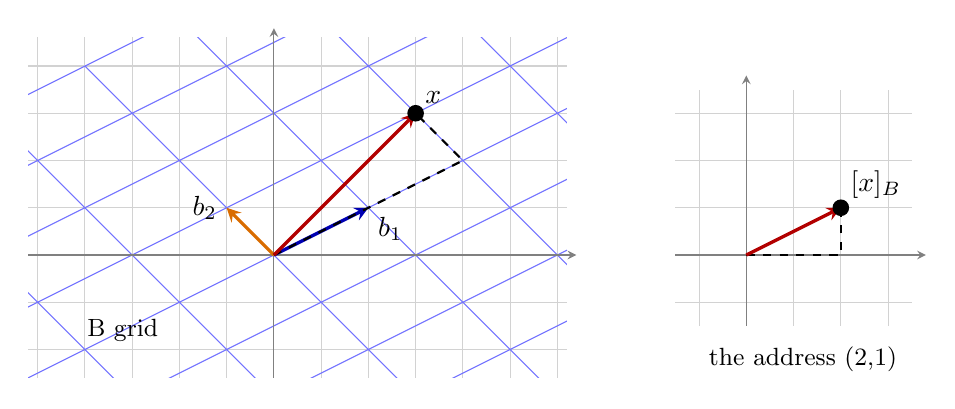
\begin{tikzpicture}[x=0.6cm,y=0.6cm,>=stealth]
  \begin{scope}
    \clip (-5.2,-2.6) rectangle (6.2,4.6);
    \draw[gray!35] (-6,-3) grid[step=1] (7,5);
    \begin{scope}[cm={2,1,-1,1,(0,0)}]
      \draw[blue!55] (-4,-4) grid[step=1] (4,4);
    \end{scope}
  \end{scope}
  \draw[->,gray] (-5.2,0)--(6.4,0);
  \draw[->,gray] (0,-2.6)--(0,4.8);
  \draw[->,very thick,blue!70!black] (0,0)--(2,1);
  \draw[->,very thick,orange!85!black] (0,0)--(-1,1);
  \draw[dashed,thick] (0,0)--(4,2)--(3,3);
  \draw[->,very thick,red!70!black] (0,0)--(3,3);
  \fill (3,3) circle (3pt);
  \node[below right] at (2,1) {$b_1$};
  \node[left] at (-1,1) {$b_2$};
  \node[above right] at (3,3) {$x$};
  \node at (-3.2,-1.6) {\small B grid};
  \begin{scope}[shift={(10,0)}]
    \draw[gray!35] (-1.5,-1.5) grid[step=1] (3.5,3.5);
    \draw[->,gray] (-1.5,0)--(3.8,0);
    \draw[->,gray] (0,-1.5)--(0,3.8);
    \draw[dashed,thick] (0,0)--(2,0)--(2,1);
    \draw[->,very thick,red!70!black] (0,0)--(2,1);
    \fill (2,1) circle (3pt);
    \node[above right] at (2,1) {$[x]_B$};
    \node at (1.2,-2.2) {\small the address (2,1)};
  \end{scope}
\end{tikzpicture}
\end{center}

\textbf{Figure 1.} One vector, two descriptions. Left: the standard grid (gray) and the grid of the basis $\mathcal{B}=\{\bv{b}_1,\bv{b}_2\}$ of Example~\ref{ex:fromB2} (blue), whose lines are the sets of vectors with one coordinate fixed. The vector $\bv{x}=2\bv{b}_1+\bv{b}_2=(3,3)$ is reached by two steps along $\bv{b}_1$ (dashed) and one step along $\bv{b}_2$. Right: its coordinate vector $[\bv{x}]_{\mathcal{B}}=(2,1)$ on ordinary graph paper. The coordinate mapping replaces the tilted grid by the square one.

\begin{exmp}{The order matters}{order}
Let $\mathcal{B}=\{\bv{b}_1,\bv{b}_2\}$ be the basis of Example~\ref{ex:fromB2} and $\mathcal{C}=\{\bv{b}_2,\bv{b}_1\}$ the same vectors in the opposite order. For $\bv{x}=(4,5)$ we found $[\bv{x}]_{\mathcal{B}}=(3,2)$, that is $\bv{x}=3\bv{b}_1+2\bv{b}_2$. Written with the vectors of $\mathcal{C}$ in order, $\bv{x}=2\bv{b}_2+3\bv{b}_1$, so $[\bv{x}]_{\mathcal{C}}=(2,3)$. Swapping $\bv{b}_1$ and $\bv{b}_2$ swapped the entries. With three vectors, let $\mathcal{B}$ be the basis of Example~\ref{ex:fromB3}, $\bv{x}=(5,1,2)$ with $[\bv{x}]_{\mathcal{B}}=(2,-1,3)$, and let $\mathcal{D}=\{\bv{b}_3,\bv{b}_1,\bv{b}_2\}$. Then $\bv{x}=3\bv{b}_3+2\bv{b}_1-1\bv{b}_2$ gives $[\bv{x}]_{\mathcal{D}}=(3,2,-1)$. In general, reordering the basis permutes the entries of the coordinate vector in the same way.
\end{exmp}

\begin{warn}[Same numbers different vectors]
A list of numbers is not a vector until we are told which basis it refers to. The coordinate vector $(3,2)$ names the vector $(3,2)$ in the standard basis, the vector $(4,5)$ in the basis $\mathcal{B}$ of Example~\ref{ex:fromB2}, and a third vector in another basis; and a vector $\bv{x}$ has a different coordinate vector in each basis. When two coordinate vectors are compared, check first that they refer to the same ordered basis.
\end{warn}

\begin{exmp}{Same numbers, different vectors; same vector, different numbers}{samenums}
Take the three bases of $\R^2$: the standard basis $\mathcal{E}$, the basis $\mathcal{B}=\{(2,1),(-1,1)\}$ and the basis $\mathcal{D}=\{(1,1),(1,-1)\}$.

\textbf{(a) The numbers $(3,2)$.} If $(3,2)$ is read as a coordinate vector, then in $\mathcal{E}$ it names $3(1,0)+2(0,1)=(3,2)$; in $\mathcal{B}$ it names $3(2,1)+2(-1,1)=(4,5)$; in $\mathcal{D}$ it names $3(1,1)+2(1,-1)=(5,1)$. Three different vectors.

\textbf{(b) The vector $(4,5)$.} Its coordinate vectors are $(4,5)$ in $\mathcal{E}$, $(3,2)$ in $\mathcal{B}$ (Example~\ref{ex:toB2}), and in $\mathcal{D}$ the solution of $c_1+c_2=4$, $c_1-c_2=5$, namely $c_1=\tfrac92$, $c_2=-\tfrac12$: $[\bv{x}]_{\mathcal{D}}=(\tfrac92,-\tfrac12)$. Check: $\tfrac92(1,1)-\tfrac12(1,-1)=(4,5)$. \ $\checkmark$ One vector, three coordinate vectors.
\end{exmp}

\begin{exmp}{The coordinates of the basis vectors}{bj}
In any basis $\mathcal{B}=\{\bv{b}_1,\dots,\bv{b}_p\}$ the basis vector $\bv{b}_j$ is $0\bv{b}_1+\cdots+1\bv{b}_j+\cdots+0\bv{b}_p$, and by uniqueness this is the only representation. So $[\bv{b}_j]_{\mathcal{B}}=\bv{e}_j$, the $j$th column of the identity matrix. In Example~\ref{ex:fromB2}, $[\bv{b}_1]_{\mathcal{B}}=(1,0)$ and $[\bv{b}_2]_{\mathcal{B}}=(0,1)$ (in the grid of Figure~1 the vector $\bv{b}_1$ is one step along the first grid direction). In $\mathbb{P}_2$ with the basis $\{1,1+t,(1+t)^2\}$ the middle basis vector has $[1+t]=(0,1,0)$. In every coordinate system the basis becomes the standard basis.
\end{exmp}

\begin{kc}{Coordinates by inspection}{inspect}
(a)~Let $\mathcal{B}=\{(1,0),(0,3)\}$. Find $[\bv{x}]_{\mathcal{B}}$ for $\bv{x}=(4,6)$. (b)~Let $\mathcal{B}=\{(1,0,0),(1,1,0),(1,1,1)\}$ and $\bv{x}=(3,2,1)$. Find $[\bv{x}]_{\mathcal{B}}$ by solving from the last coordinate up. (c)~In $\mathbb{P}_2$ with the standard basis $\{1,t,t^2\}$, find $[7-t^2]$. (d)~If $[\bv{x}]_{\mathcal{B}}=(5,6,7)$ for $\mathcal{B}=\{\bv{b}_1,\bv{b}_2,\bv{b}_3\}$, find $[\bv{x}]_{\mathcal{C}}$ for $\mathcal{C}=\{\bv{b}_3,\bv{b}_1,\bv{b}_2\}$.
\end{kc}

% ---------------------------------------------------------------------
\subsection*{Coordinates in $\R^n$: the matrix $P_{\mathcal{B}}$}

Equation $\bv{x}=c_1\bv{b}_1+\cdots+c_p\bv{b}_p$ is a matrix-vector product (Definition~\ref{1.4-def:matvec}). Let $\mathcal{B}=\{\bv{b}_1,\dots,\bv{b}_p\}$ be a basis for a subspace of $\R^n$ and put
\[
P_{\mathcal{B}}=\begin{bmatrix}\bv{b}_1&\bv{b}_2&\cdots&\bv{b}_p\end{bmatrix},
\]
an $n\times p$ matrix. Then, for every $\bv{x}$ in the subspace,
\[
\bv{x}=P_{\mathcal{B}}\,[\bv{x}]_{\mathcal{B}}.
\]
Nothing is assumed here about $p$. In all our examples of a basis for $\R^n$ the number of vectors is $n$, so $P_{\mathcal{B}}$ is square; this is the case in which the matrix can be inverted. (Whether it must always be so is the question left open in Pause and think~\ref{4.3-think:manybases}; we do not need the answer.)

\begin{thm}{Coordinates in $\R^n$}{PB}
Let $\mathcal{B}=\{\bv{b}_1,\dots,\bv{b}_n\}$ be a basis for $\R^n$ consisting of $n$ vectors. Then $P_{\mathcal{B}}$ is an invertible $n\times n$ matrix, and for every $\bv{x}$ in $\R^n$
\[
\bv{x}=P_{\mathcal{B}}[\bv{x}]_{\mathcal{B}},\qquad [\bv{x}]_{\mathcal{B}}=P_{\mathcal{B}}^{-1}\bv{x}.
\]
\end{thm}

\begin{proof}
The columns of $P_{\mathcal{B}}$ are independent and span $\R^n$ because $\mathcal{B}$ is a basis, so $P_{\mathcal{B}}$ is a square matrix satisfying statements (e) and (h) of the Invertible Matrix Theorem (Theorem~\ref{2.3-thm:imt}); hence it is invertible. The equation $\bv{x}=P_{\mathcal{B}}[\bv{x}]_{\mathcal{B}}$ was shown above. Multiplying it on the left by $P_{\mathcal{B}}^{-1}$ gives $[\bv{x}]_{\mathcal{B}}=P_{\mathcal{B}}^{-1}\bv{x}$ (Theorem~\ref{2.2-thm:solve}).
\end{proof}

\begin{think}{Which statements of the Invertible Matrix Theorem?}{square}
In the proof of Theorem~\ref{thm:PB} the matrix $P_{\mathcal{B}}$ is square and has two properties because $\mathcal{B}$ is a basis. (a)~Name them, and (b)~name the statements of Theorem~\ref{2.3-thm:imt} to which they correspond. (c)~The Invertible Matrix Theorem is about square matrices. If $P_{\mathcal{B}}$ were not square, could it have an inverse? Which of the two formulas $\bv{x}=P_{\mathcal{B}}[\bv{x}]_{\mathcal{B}}$ and $[\bv{x}]_{\mathcal{B}}=P_{\mathcal{B}}^{-1}\bv{x}$ would survive?
\end{think}

\begin{exmp}{$P_{\mathcal{B}}$ and its inverse in $\R^2$}{PB2}
For $\mathcal{B}=\{(2,1),(-1,1)\}$,
\[
P_{\mathcal{B}}=\begin{bmatrix}2&-1\\1&1\end{bmatrix},\qquad \det P_{\mathcal{B}}=2+1=3,\qquad P_{\mathcal{B}}^{-1}=\begin{bmatrix}\tfrac13&\tfrac13\\-\tfrac13&\tfrac23\end{bmatrix}
\]
by the formula of Theorem~\ref{2.2-thm:twobytwo}. Check:
\[
\begin{bmatrix}2&-1\\1&1\end{bmatrix}\begin{bmatrix}\tfrac13&\tfrac13\\-\tfrac13&\tfrac23\end{bmatrix}=\begin{bmatrix}1&0\\0&1\end{bmatrix}.
\]
Now $P_{\mathcal{B}}$ and $P_{\mathcal{B}}^{-1}$ do the two directions at once. From coordinates to the vector:
\[
\begin{bmatrix}2&-1\\1&1\end{bmatrix}\begin{bmatrix}3\\2\end{bmatrix}=\begin{bmatrix}4\\5\end{bmatrix}.
\]
From the vector to coordinates, for the three vectors $(4,5)$, $(1,0)$, $(-3,0)$:
\[
\begin{bmatrix}\tfrac13&\tfrac13\\-\tfrac13&\tfrac23\end{bmatrix}\begin{bmatrix}4\\5\end{bmatrix}=\begin{bmatrix}3\\2\end{bmatrix},\qquad
\begin{bmatrix}\tfrac13&\tfrac13\\-\tfrac13&\tfrac23\end{bmatrix}\begin{bmatrix}1\\0\end{bmatrix}=\begin{bmatrix}\tfrac13\\-\tfrac13\end{bmatrix},\qquad
\begin{bmatrix}\tfrac13&\tfrac13\\-\tfrac13&\tfrac23\end{bmatrix}\begin{bmatrix}-3\\0\end{bmatrix}=\begin{bmatrix}-1\\1\end{bmatrix}.
\]
The first and third agree with Example~\ref{ex:toB2}. The inverse is computed once and then used for every $\bv{x}$ (compare Pause and think~\ref{2.2-think:manyb}): that is the advantage of $P_{\mathcal{B}}^{-1}$ over row reducing $[\,P_{\mathcal{B}}\ \bv{x}\,]$ separately each time. The coordinates of $(1,0)$ are fractions; a vector with integer entries can have non-integer coordinates.
\end{exmp}

\begin{exmp}{$P_{\mathcal{B}}$ and its inverse in $\R^3$}{PB3}
For $\mathcal{B}=\{(1,1,0),(0,1,1),(1,0,1)\}$,
\[
P_{\mathcal{B}}=\begin{bmatrix}1&0&1\\1&1&0\\0&1&1\end{bmatrix}.
\]
Row reduce $[\,P_{\mathcal{B}}\ I\,]$ (Theorem~\ref{2.2-thm:algorithm}):
\begin{align*}
\begin{amat}{ccc|ccc}1 & 0 & 1 & 1 & 0 & 0\\1 & 1 & 0 & 0 & 1 & 0\\0 & 1 & 1 & 0 & 0 & 1\end{amat}
&\rops{R_2-R_1}
\begin{amat}{ccc|ccc}1 & 0 & 1 & 1 & 0 & 0\\0 & 1 & -1 & -1 & 1 & 0\\0 & 1 & 1 & 0 & 0 & 1\end{amat}
\\[4pt]
&\rops{R_3-R_2}
\begin{amat}{ccc|ccc}1 & 0 & 1 & 1 & 0 & 0\\0 & 1 & -1 & -1 & 1 & 0\\0 & 0 & 2 & 1 & -1 & 1\end{amat}
\\[4pt]
&\rops{\tfrac{1}{2}R_3}
\begin{amat}{ccc|ccc}1 & 0 & 1 & 1 & 0 & 0\\0 & 1 & -1 & -1 & 1 & 0\\0 & 0 & 1 & \tfrac{1}{2} & -\tfrac{1}{2} & \tfrac{1}{2}\end{amat}
\\[4pt]
&\rops{R_2+R_3}
\begin{amat}{ccc|ccc}1 & 0 & 1 & 1 & 0 & 0\\0 & 1 & 0 & -\tfrac{1}{2} & \tfrac{1}{2} & \tfrac{1}{2}\\0 & 0 & 1 & \tfrac{1}{2} & -\tfrac{1}{2} & \tfrac{1}{2}\end{amat}
\\[4pt]
&\rops{R_1-R_3}
\begin{amat}{ccc|ccc}1 & 0 & 0 & \tfrac{1}{2} & \tfrac{1}{2} & -\tfrac{1}{2}\\0 & 1 & 0 & -\tfrac{1}{2} & \tfrac{1}{2} & \tfrac{1}{2}\\0 & 0 & 1 & \tfrac{1}{2} & -\tfrac{1}{2} & \tfrac{1}{2}\end{amat}
\end{align*}
Hence
\[
P_{\mathcal{B}}^{-1}=\begin{bmatrix}\tfrac12&\tfrac12&-\tfrac12\\-\tfrac12&\tfrac12&\tfrac12\\\tfrac12&-\tfrac12&\tfrac12\end{bmatrix},\qquad
\begin{bmatrix}\tfrac12&\tfrac12&-\tfrac12\\-\tfrac12&\tfrac12&\tfrac12\\\tfrac12&-\tfrac12&\tfrac12\end{bmatrix}\begin{bmatrix}3\\1\\2\end{bmatrix}=\begin{bmatrix}1\\0\\2\end{bmatrix}.
\]
The second equation says again that $[\bv{x}]_{\mathcal{B}}=(1,0,2)$ for $\bv{x}=(3,1,2)$ (Example~\ref{ex:toB3}). The first equation is verified by the product $P_{\mathcal{B}}P_{\mathcal{B}}^{-1}=I$:
\[
\begin{bmatrix}1&0&1\\1&1&0\\0&1&1\end{bmatrix}\begin{bmatrix}\tfrac12&\tfrac12&-\tfrac12\\-\tfrac12&\tfrac12&\tfrac12\\\tfrac12&-\tfrac12&\tfrac12\end{bmatrix}=\begin{bmatrix}1&0&0\\0&1&0\\0&0&1\end{bmatrix}.
\]
\end{exmp}

\begin{exmp}{A triangular basis: no row reduction needed}{tri}
Let $\mathcal{B}=\{(1,0,0),(1,1,0),(1,1,1)\}$. Then $P_{\mathcal{B}}$ is upper triangular with ones on the diagonal (Theorem~\ref{2.3-thm:triangular}), so $\mathcal{B}$ is a basis, and
\[
P_{\mathcal{B}}=\begin{bmatrix}1&1&1\\0&1&1\\0&0&1\end{bmatrix},\qquad
P_{\mathcal{B}}^{-1}=\begin{bmatrix}1&-1&0\\0&1&-1\\0&0&1\end{bmatrix},\qquad
\begin{bmatrix}1&1&1\\0&1&1\\0&0&1\end{bmatrix}\begin{bmatrix}1&-1&0\\0&1&-1\\0&0&1\end{bmatrix}=\begin{bmatrix}1&0&0\\0&1&0\\0&0&1\end{bmatrix}.
\]
For $\bv{x}=(5,3,1)$ the coordinates are $[\bv{x}]_{\mathcal{B}}=P_{\mathcal{B}}^{-1}\bv{x}=(5-3,\ 3-1,\ 1)=(2,2,1)$. Check by building: $2(1,0,0)+2(1,1,0)+1(1,1,1)=(5,3,1)$. \ $\checkmark$ In general $[\bv{x}]_{\mathcal{B}}=(x_1-x_2,\ x_2-x_3,\ x_3)$ for this basis: a good choice of basis makes the coordinates easy to compute.
\end{exmp}

\begin{kc}{The matrix $P_{\mathcal{B}}$}{PB}
Let $\mathcal{B}=\{(1,2),(3,5)\}$. (a)~Write $P_{\mathcal{B}}$ and find $P_{\mathcal{B}}^{-1}$ with the $2\times2$ formula. (b)~Use it to find $[\bv{x}]_{\mathcal{B}}$ for $\bv{x}=(1,1)$ and check by building $\bv{x}$ from $\mathcal{B}$. (c)~Which of the two matrices, $P_{\mathcal{B}}$ or $P_{\mathcal{B}}^{-1}$, multiplies a coordinate vector to give a vector, and which does the reverse?
\end{kc}

% ---------------------------------------------------------------------
\subsection*{The coordinate mapping}

The coordinate mapping connects a possibly unfamiliar space $V$ with the familiar space $\R^p$. What does it preserve? Everything that is built from addition and scalar multiplication.

\begin{thm}{The coordinate mapping is linear, one-to-one and onto}{coordmap}
Let $\mathcal{B}=\{\bv{b}_1,\dots,\bv{b}_p\}$ be a basis for a vector space $V$. The coordinate mapping $\bv{x}\mapsto[\bv{x}]_{\mathcal{B}}$ is a linear transformation from $V$ to $\R^p$ (Definition~\ref{4.2-def:lintrans}) that is one-to-one and onto $\R^p$. In particular, for all $\bv{u}_1,\dots,\bv{u}_k$ in $V$ and scalars $c_1,\dots,c_k$,
\[
[c_1\bv{u}_1+\cdots+c_k\bv{u}_k]_{\mathcal{B}}=c_1[\bv{u}_1]_{\mathcal{B}}+\cdots+c_k[\bv{u}_k]_{\mathcal{B}}.
\]
\end{thm}

\begin{proof}
\emph{Linear.} Let $\bv{u}=c_1\bv{b}_1+\cdots+c_p\bv{b}_p$ and $\bv{w}=d_1\bv{b}_1+\cdots+d_p\bv{b}_p$ be two vectors of $V$. By the vector space axioms $\bv{u}+\bv{w}=(c_1+d_1)\bv{b}_1+\cdots+(c_p+d_p)\bv{b}_p$, and by uniqueness this is the representation of $\bv{u}+\bv{w}$, so
\[
[\bv{u}+\bv{w}]_{\mathcal{B}}=\begin{bmatrix}c_1+d_1\\\vdots\\c_p+d_p\end{bmatrix}=[\bv{u}]_{\mathcal{B}}+[\bv{w}]_{\mathcal{B}}.
\]
For a scalar $r$, $r\bv{u}=(rc_1)\bv{b}_1+\cdots+(rc_p)\bv{b}_p$, so $[r\bv{u}]_{\mathcal{B}}=r[\bv{u}]_{\mathcal{B}}$. The displayed formula for $k$ vectors follows by repeating these two rules, as in Theorem~\ref{1.8-thm:props}.

\emph{One-to-one.} If $[\bv{u}]_{\mathcal{B}}=[\bv{w}]_{\mathcal{B}}$, then the weights are equal, so $\bv{u}=c_1\bv{b}_1+\cdots+c_p\bv{b}_p=\bv{w}$.

\emph{Onto.} Given $\bv{y}=(y_1,\dots,y_p)$ in $\R^p$, the vector $\bv{x}=y_1\bv{b}_1+\cdots+y_p\bv{b}_p$ is in $V$, and by uniqueness $[\bv{x}]_{\mathcal{B}}=\bv{y}$.
\end{proof}

A one-to-one linear map of $V$ \emph{onto} a vector space $W$ is called an \emph{isomorphism} from $V$ to $W$; the theorem says that the coordinate mapping is an isomorphism from $V$ onto $\R^p$. (We do not draw any conclusion here beyond what is proved: the coordinate mapping matches the vectors of $V$ with those of $\R^p$ one for one and preserves sums and scalar multiples.) For $V=\R^n$ and $p=n$ the coordinate mapping is the matrix transformation $\bv{x}\mapsto P_{\mathcal{B}}^{-1}\bv{x}$, which is linear by Theorem~\ref{1.8-thm:matlin}: the theorem agrees with Theorem~\ref{thm:PB}.

\begin{exmp}{Checking linearity on numbers}{lincheck}
Let $\mathcal{B}=\{(2,1),(-1,1)\}$, $\bv{u}=(4,5)$, $\bv{w}=(1,0)$. From Example~\ref{ex:PB2}: $[\bv{u}]_{\mathcal{B}}=(3,2)$ and $[\bv{w}]_{\mathcal{B}}=(\tfrac13,-\tfrac13)$. Then
\[
\bv{u}+\bv{w}=(5,5):\ \ [\bv{u}+\bv{w}]_{\mathcal{B}}=P_{\mathcal{B}}^{-1}\begin{bmatrix}5\\5\end{bmatrix}=\begin{bmatrix}\tfrac{10}{3}\\\tfrac53\end{bmatrix}=\begin{bmatrix}3\\2\end{bmatrix}+\begin{bmatrix}\tfrac13\\-\tfrac13\end{bmatrix}=[\bv{u}]_{\mathcal{B}}+[\bv{w}]_{\mathcal{B}},
\]
and for the combination $2\bv{u}-3\bv{w}=(8,10)-(3,0)=(5,10)$:
\[
[2\bv{u}-3\bv{w}]_{\mathcal{B}}=P_{\mathcal{B}}^{-1}\begin{bmatrix}5\\10\end{bmatrix}=\begin{bmatrix}5\\5\end{bmatrix}=2\begin{bmatrix}3\\2\end{bmatrix}-3\begin{bmatrix}\tfrac13\\-\tfrac13\end{bmatrix}.
\]
Both sides of the second equation equal $(5,5)$ since $2(3,2)-3(\tfrac13,-\tfrac13)=(6,4)-(1,-1)$. The coordinate mapping respects sums and scalar multiples, as Theorem~\ref{thm:coordmap} promises.
\end{exmp}

\begin{exmp}{Maps built from coordinates that are not linear}{notlin}
Keep $\mathcal{B}=\{(2,1),(-1,1)\}$, and write $[\bv{x}]_{\mathcal{B}}=(c_1,c_2)$. Three maps $\R^2\to\R^2$ or $\R^2\to\R$ are defined from the coordinates; test each with the vectors $\bv{u}=(4,5)$ (with $[\bv{u}]_{\mathcal{B}}=(3,2)$) and $2\bv{u}=(8,10)$ (with $[2\bv{u}]_{\mathcal{B}}=(6,4)$).

\textbf{(a) Squaring the coordinates.} $S(\bv{x})=(c_1^2,c_2^2)$. Then $S(\bv{u})=(9,4)$ and $S(2\bv{u})=(36,16)$, but $2S(\bv{u})=(18,8)$. The scalar rule fails, so $S$ is not linear. (The coordinate mapping is linear, but squaring its output is not.)

\textbf{(b) Shifting the coordinates.} $T(\bv{x})=(c_1+1,\ c_2)$. Here $T(\bv{0})=(1,0)\neq\bv{0}$, so $T$ is not linear (Theorem~\ref{1.8-thm:props}(a)).

\textbf{(c) Multiplying the coordinates.} $U(\bv{x})=c_1c_2$. Then $U(\bv{u})=6$ and $U(2\bv{u})=24\neq12=2U(\bv{u})$: not linear.

\textbf{(d) A linear one.} $V(\bv{x})=c_2$, the second coordinate. With $\bv{w}=(1,0)$, $[\bv{w}]_{\mathcal{B}}=(\tfrac13,-\tfrac13)$ we get $V(\bv{u})=2$, $V(\bv{w})=-\tfrac13$, $V(\bv{u}+\bv{w})=\tfrac53=2-\tfrac13$ and $V(2\bv{u})=4=2V(\bv{u})$, as it should: $V$ is the composition of the linear coordinate mapping with the linear map ``pick the second entry''. Numerical tests like these can show that a map is \emph{not} linear (one failed instance suffices) but never prove that it is.
\end{exmp}

\begin{think}{What does the coordinate mapping not preserve?}{notpreserved}
The coordinate mapping preserves sums and scalar multiples. (a)~Does it preserve the entries of a vector? Compare $\bv{x}=(4,5)$ and $[\bv{x}]_{\mathcal{B}}=(3,2)$. (b)~If $\bv{x}$ has all entries positive, must $[\bv{x}]_{\mathcal{B}}$ have all entries positive? Use $(1,0)$ and the basis $\mathcal{B}=\{(2,1),(-1,1)\}$. (c)~Which of the two statements ``$\bv{u}$ is a sum of $\bv{v}$ and $\bv{w}$'' and ``$\bv{u}$ has positive entries'' can be tested in coordinates?
\end{think}

% ---------------------------------------------------------------------
\subsection*{Moving questions into $\R^p$}

Because the coordinate mapping is linear, one-to-one and onto, any question that is built from linear combinations can be moved to $\R^p$, answered there by row reduction, and moved back.

\begin{thm}{Questions answered in coordinates}{transfer}
Let $\mathcal{B}$ be a basis for $V$ with $p$ vectors, and let $\bv{u}_1,\dots,\bv{u}_k$ and $\bv{w}$ be vectors in $V$.
\begin{enumerate}[label=(\alph*),itemsep=1pt]
  \item $c_1\bv{u}_1+\cdots+c_k\bv{u}_k=\bv{w}$ if and only if $c_1[\bv{u}_1]_{\mathcal{B}}+\cdots+c_k[\bv{u}_k]_{\mathcal{B}}=[\bv{w}]_{\mathcal{B}}$. Hence $\bv{w}$ is in $\Span\{\bv{u}_1,\dots,\bv{u}_k\}$ if and only if $[\bv{w}]_{\mathcal{B}}$ is in $\Span\{[\bv{u}_1]_{\mathcal{B}},\dots,[\bv{u}_k]_{\mathcal{B}}\}$, with the same weights.
  \item $\{\bv{u}_1,\dots,\bv{u}_k\}$ is linearly independent in $V$ if and only if $\{[\bv{u}_1]_{\mathcal{B}},\dots,[\bv{u}_k]_{\mathcal{B}}\}$ is linearly independent in $\R^p$; a dependence relation among the $\bv{u}_i$ has the same weights as the one among their coordinate vectors.
  \item $\{\bv{u}_1,\dots,\bv{u}_k\}$ spans $V$ if and only if $\{[\bv{u}_1]_{\mathcal{B}},\dots,[\bv{u}_k]_{\mathcal{B}}\}$ spans $\R^p$.
  \item $\{\bv{u}_1,\dots,\bv{u}_k\}$ is a basis for $V$ if and only if $\{[\bv{u}_1]_{\mathcal{B}},\dots,[\bv{u}_k]_{\mathcal{B}}\}$ is a basis for $\R^p$.
\end{enumerate}
\end{thm}

\begin{proof}
(a)~By Theorem~\ref{thm:coordmap}, $[c_1\bv{u}_1+\cdots+c_k\bv{u}_k]_{\mathcal{B}}=c_1[\bv{u}_1]_{\mathcal{B}}+\cdots+c_k[\bv{u}_k]_{\mathcal{B}}$, and since the mapping is one-to-one, the vectors $c_1\bv{u}_1+\cdots+c_k\bv{u}_k$ and $\bv{w}$ are equal exactly when their coordinate vectors are equal. (b)~Take $\bv{w}=\bv{0}$ in (a): $[\bv{0}]_{\mathcal{B}}=\bv{0}$ because $\bv{0}=0\bv{b}_1+\cdots+0\bv{b}_p$. So $c_1\bv{u}_1+\cdots+c_k\bv{u}_k=\bv{0}$ has the same solutions $(c_1,\dots,c_k)$ as $c_1[\bv{u}_1]_{\mathcal{B}}+\cdots+c_k[\bv{u}_k]_{\mathcal{B}}=\bv{0}$, so one equation has only the trivial solution exactly when the other does. (c)~If the $\bv{u}_i$ span $V$ and $\bv{y}$ is in $\R^p$, then $\bv{y}=[\bv{x}]_{\mathcal{B}}$ for some $\bv{x}$ (onto), $\bv{x}=\sum c_i\bv{u}_i$, so $\bv{y}=\sum c_i[\bv{u}_i]_{\mathcal{B}}$. Conversely if the coordinate vectors span $\R^p$ and $\bv{x}$ is in $V$, write $[\bv{x}]_{\mathcal{B}}=\sum c_i[\bv{u}_i]_{\mathcal{B}}$; by (a), $\bv{x}=\sum c_i\bv{u}_i$. (d)~is (b) together with (c).
\end{proof}

\begin{proc}{Testing polynomials, matrices and functions by coordinates}{testcoords}
\begin{enumerate}
  \item Choose a basis $\mathcal{B}$ for the space (usually the standard one) and write each vector as a coordinate column.
  \item Make the matrix whose columns are the coordinate vectors.
  \item Row reduce. \emph{Independent}: a pivot in every column. \emph{Spanning}: a pivot in every row. \emph{Basis}: both. \emph{In the span}: no pivot in the last column of $[\,\text{columns}\ \ [\bv{w}]\,]$.
  \item Translate the answer back to the polynomials, matrices or functions, including any weights.
\end{enumerate}
\end{proc}

% ---------------------------------------------------------------------
\subsection*{Coordinates in $\mathbb{P}_n$, $M_{2\times2}$ and spaces of functions}

For vector spaces other than $\R^n$ the coordinate mapping is the way to turn a question about polynomials, matrices or functions into a question about columns of numbers. The easiest basis to use is the standard one, and then the coordinates are the coefficients or entries.

\begin{exmp}{Standard coordinates in $\mathbb{P}_2$}{P2std}
In $\mathbb{P}_2$ with the standard basis $\mathcal{E}=\{1,t,t^2\}$ (Example~\ref{4.3-ex:standard}),
\[
[3-2t+5t^2]_{\mathcal{E}}=\begin{bmatrix}3\\-2\\5\end{bmatrix},\qquad [t^2-1]_{\mathcal{E}}=\begin{bmatrix}-1\\0\\1\end{bmatrix},\qquad [t]_{\mathcal{E}}=\begin{bmatrix}0\\1\\0\end{bmatrix}.
\]
Adding polynomials adds their coefficient columns, and $[(3-2t+5t^2)+(t^2-1)]_{\mathcal{E}}=[2-2t+6t^2]_{\mathcal{E}}=(2,-2,6)=(3,-2,5)+(-1,0,1)$. This is the identification of polynomials with coefficient vectors that we used in Example~\ref{1.8-ex:poly}, now seen as the coordinate mapping for the standard basis.
\end{exmp}

\begin{exmp}{A nonstandard basis of $\mathbb{P}_2$}{P2taylor}
Let $\mathcal{B}=\{1,\ 1+t,\ (1+t)^2\}$. Since $(1+t)^2=1+2t+t^2$, the standard coordinates of the basis vectors are $(1,0,0)$, $(1,1,0)$, $(1,2,1)$. These are independent and span $\R^3$ (the matrix is triangular with ones on the diagonal, as in Example~\ref{ex:tri}), so $\mathcal{B}$ is a basis for $\mathbb{P}_2$ by Theorem~\ref{thm:transfer}(d). Find $[p]_{\mathcal{B}}$ for $p=2-3t+t^2$.

\textbf{Solution.} Work with the standard coordinates of the three basis polynomials and of $p$:
\begin{align*}
\begin{amat}{ccc|c}1 & 1 & 1 & 2\\0 & 1 & 2 & -3\\0 & 0 & 1 & 1\end{amat}
&\rops{R_2-2R_3}
\begin{amat}{ccc|c}1 & 1 & 1 & 2\\0 & 1 & 0 & -5\\0 & 0 & 1 & 1\end{amat}
\rops{R_1-R_3}
\begin{amat}{ccc|c}1 & 1 & 0 & 1\\0 & 1 & 0 & -5\\0 & 0 & 1 & 1\end{amat}
\\[4pt]
&\rops{R_1-R_2}
\begin{amat}{ccc|c}1 & 0 & 0 & 6\\0 & 1 & 0 & -5\\0 & 0 & 1 & 1\end{amat}
\end{align*}
so $[p]_{\mathcal{B}}=(6,-5,1)$. Check: $6\cdot1-5(1+t)+1(1+2t+t^2)=(6-5+1)+(-5+2)t+t^2=2-3t+t^2$. \ $\checkmark$ In the notation of the previous section, $P_{\mathcal{B}}$ here is the matrix of the standard coordinates of the basis, $P_{\mathcal{B}}=\begin{bmatrix}1&1&1\\0&1&2\\0&0&1\end{bmatrix}$ with inverse $P_{\mathcal{B}}^{-1}=\begin{bmatrix}1&-1&1\\0&1&-2\\0&0&1\end{bmatrix}$:
\[
\begin{bmatrix}1&1&1\\0&1&2\\0&0&1\end{bmatrix}\begin{bmatrix}1&-1&1\\0&1&-2\\0&0&1\end{bmatrix}=\begin{bmatrix}1&0&0\\0&1&0\\0&0&1\end{bmatrix},\qquad
\begin{bmatrix}1&-1&1\\0&1&-2\\0&0&1\end{bmatrix}\begin{bmatrix}2\\-3\\1\end{bmatrix}=\begin{bmatrix}6\\-5\\1\end{bmatrix}.
\]
The columns of $P_{\mathcal{B}}^{-1}$ are the coordinates of $1$, $t$, $t^2$ relative to $\mathcal{B}$: $t=-1+(1+t)$ and $t^2=1-2(1+t)+(1+t)^2$.
\end{exmp}

\begin{exmp}{From the coordinates to the polynomial; one polynomial in several bases}{whichvec}
\textbf{(a)} Which polynomial has $[p]_{\mathcal{B}}=(1,2,3)$ for the basis $\mathcal{B}$ of Example~\ref{ex:P2taylor}? Build it: $p=1\cdot1+2(1+t)+3(1+t)^2=1+2+2t+3+6t+3t^2=6+8t+3t^2$. Every list of three numbers is the coordinate vector of exactly one polynomial, which is what ``onto'' and ``one-to-one'' say.

\textbf{(b)} The polynomial $p=t^2$ has standard coordinates $(0,0,1)$; relative to $\mathcal{B}$ it has $[p]_{\mathcal{B}}=(1,-2,1)$ (the third column of $P_{\mathcal{B}}^{-1}$ above); relative to the reordered standard basis $\{t^2,t,1\}$ it has $(1,0,0)$. One polynomial, three coordinate vectors.
\end{exmp}

\begin{exmp}{A nonstandard basis of $M_{2\times2}$}{M2}
Let
\[
B_1=\begin{bmatrix}1&1\\0&0\end{bmatrix},\quad B_2=\begin{bmatrix}0&1\\1&0\end{bmatrix},\quad B_3=\begin{bmatrix}0&0\\1&1\end{bmatrix},\quad B_4=\begin{bmatrix}1&0\\0&0\end{bmatrix},
\]
and $\mathcal{B}=\{B_1,B_2,B_3,B_4\}$. Using the standard coordinates $(a_{11},a_{12},a_{21},a_{22})$ of a matrix (the entries read row by row, Example~\ref{4.3-ex:standard}), find $[A]_{\mathcal{B}}$ for $A=\begin{bmatrix}4&3\\2&1\end{bmatrix}$, and $A$ if $[A]_{\mathcal{B}}=(1,-1,2,0)$.

\textbf{Solution.} The columns are the standard coordinates $(1,1,0,0)$, $(0,1,1,0)$, $(0,0,1,1)$, $(1,0,0,0)$ of $B_1,\dots,B_4$, and the last column is $(4,3,2,1)$:
\begin{align*}
\begin{amat}{cccc|c}1 & 0 & 0 & 1 & 4\\1 & 1 & 0 & 0 & 3\\0 & 1 & 1 & 0 & 2\\0 & 0 & 1 & 0 & 1\end{amat}
&\rops{R_2-R_1}
\begin{amat}{cccc|c}1 & 0 & 0 & 1 & 4\\0 & 1 & 0 & -1 & -1\\0 & 1 & 1 & 0 & 2\\0 & 0 & 1 & 0 & 1\end{amat}
\\[4pt]
&\rops{R_3-R_2}
\begin{amat}{cccc|c}1 & 0 & 0 & 1 & 4\\0 & 1 & 0 & -1 & -1\\0 & 0 & 1 & 1 & 3\\0 & 0 & 1 & 0 & 1\end{amat}
\\[4pt]
&\rops{R_4-R_3}
\begin{amat}{cccc|c}1 & 0 & 0 & 1 & 4\\0 & 1 & 0 & -1 & -1\\0 & 0 & 1 & 1 & 3\\0 & 0 & 0 & -1 & -2\end{amat}
\\[4pt]
&\rops{-R_4}
\begin{amat}{cccc|c}1 & 0 & 0 & 1 & 4\\0 & 1 & 0 & -1 & -1\\0 & 0 & 1 & 1 & 3\\0 & 0 & 0 & 1 & 2\end{amat}
\\[4pt]
&\rops{R_3-R_4}
\begin{amat}{cccc|c}1 & 0 & 0 & 1 & 4\\0 & 1 & 0 & -1 & -1\\0 & 0 & 1 & 0 & 1\\0 & 0 & 0 & 1 & 2\end{amat}
\\[4pt]
&\rops{R_2+R_4}
\begin{amat}{cccc|c}1 & 0 & 0 & 1 & 4\\0 & 1 & 0 & 0 & 1\\0 & 0 & 1 & 0 & 1\\0 & 0 & 0 & 1 & 2\end{amat}
\\[4pt]
&\rops{R_1-R_4}
\begin{amat}{cccc|c}1 & 0 & 0 & 0 & 2\\0 & 1 & 0 & 0 & 1\\0 & 0 & 1 & 0 & 1\\0 & 0 & 0 & 1 & 2\end{amat}
\end{align*}
There is a pivot in every column and in every row of the left block, so its four columns are independent and span $\R^4$, and $\mathcal{B}$ is a basis for $M_{2\times2}$ by Theorem~\ref{thm:transfer}(d). The last column is the coordinate vector: $[A]_{\mathcal{B}}=(2,1,1,2)$. Check: $2B_1+B_2+B_3+2B_4=\begin{bmatrix}2+2&2+1\\1+1&1\end{bmatrix}=\begin{bmatrix}4&3\\2&1\end{bmatrix}$. \ $\checkmark$ For the other direction no row reduction is needed: $A=1B_1-1B_2+2B_3+0B_4=\begin{bmatrix}1&1-1\\-1+2&2\end{bmatrix}=\begin{bmatrix}1&0\\1&2\end{bmatrix}$.
\end{exmp}

\begin{exmp}{Coordinates in a space of functions}{func}
Let $H=\Span\{\cos t,\sin t\}$, with the standard basis $\{\cos t,\sin t\}$ (independent by Example~\ref{4.3-ex:sincos}). Consider $\mathcal{C}=\{\cos t+\sin t,\ \cos t-\sin t\}$. Its standard coordinates are $(1,1)$ and $(1,-1)$, which are independent and span $\R^2$, so $\mathcal{C}$ is a basis for $H$ (Theorem~\ref{thm:transfer}(d), applied to $H$ with the standard basis). Find $[f]_{\mathcal{C}}$ for $f=3\cos t+\sin t$.

\textbf{Solution.} The standard coordinates of $f$ are $(3,1)$:
\begin{align*}
\begin{amat}{cc|c}1 & 1 & 3\\1 & -1 & 1\end{amat}
&\rops{R_2-R_1}
\begin{amat}{cc|c}1 & 1 & 3\\0 & -2 & -2\end{amat}
\rops{-\tfrac{1}{2}R_2}
\begin{amat}{cc|c}1 & 1 & 3\\0 & 1 & 1\end{amat}
\rops{R_1-R_2}
\begin{amat}{cc|c}1 & 0 & 2\\0 & 1 & 1\end{amat}
\end{align*}
so $[f]_{\mathcal{C}}=(2,1)$. Check: $2(\cos t+\sin t)+(\cos t-\sin t)=3\cos t+\sin t$. \ $\checkmark$ In the other direction, the function $g$ with $[g]_{\mathcal{C}}=(1,-3)$ is $g=(\cos t+\sin t)-3(\cos t-\sin t)=-2\cos t+4\sin t$. The standard coordinates did the work; the answer is a statement about functions.
\end{exmp}

\begin{exmp}{Functions times an exponential}{func3}
Let $H=\Span\{e^t,\ te^t,\ t^2e^t\}$ with the basis $\mathcal{B}=\{e^t,te^t,t^2e^t\}$ (these three functions are independent: evaluating $c_1e^t+c_2te^t+c_3t^2e^t=0$ at $t=0$ gives $c_1=0$, at $t=1$ gives $c_2+c_3=0$, at $t=-1$ gives $-c_2+c_3=0$, so $c_2=c_3=0$). For $f=(2-t+3t^2)e^t$ and $g=(t-t^2)e^t$,
\[
[f]_{\mathcal{B}}=\begin{bmatrix}2\\-1\\3\end{bmatrix},\qquad [g]_{\mathcal{B}}=\begin{bmatrix}0\\1\\-1\end{bmatrix},\qquad [f+g]_{\mathcal{B}}=[(2+2t^2)e^t]_{\mathcal{B}}=\begin{bmatrix}2\\0\\2\end{bmatrix}=[f]_{\mathcal{B}}+[g]_{\mathcal{B}}.
\]
\end{exmp}

\begin{kc}{Coordinates outside $\R^n$}{outside}
(a)~In $\mathbb{P}_2$ with $\mathcal{B}=\{1,1+t,(1+t)^2\}$, find $p$ if $[p]_{\mathcal{B}}=(2,0,-1)$. (b)~In $M_{2\times2}$ with the standard basis $\{E_{11},E_{12},E_{21},E_{22}\}$, find $[A]$ for $A=\begin{bmatrix}2&-1\\0&5\end{bmatrix}$ (Example~\ref{4.3-ex:standard}). (c)~In $H=\Span\{\cos t,\sin t\}$ with $\mathcal{C}$ from Example~\ref{ex:func}, find $[h]_{\mathcal{C}}$ for $h=\sin t$.
\end{kc}

% ---------------------------------------------------------------------
\subsection*{Worked tests in coordinates}

\begin{exmp}{Independence of polynomials in $\mathbb{P}_3$}{indepP3}
Is $\{1+2t^3,\ 2+t-3t^2,\ -t+2t^2-t^3\}$ linearly independent in $\mathbb{P}_3$?

\textbf{Solution.} The standard coordinates (coefficients of $1,t,t^2,t^3$) are $(1,0,0,2)$, $(2,1,-3,0)$, $(0,-1,2,-1)$:
\begin{align*}
\begin{amat}{ccc}1 & 2 & 0\\0 & 1 & -1\\0 & -3 & 2\\2 & 0 & -1\end{amat}
&\rops{R_4-2R_1}
\begin{amat}{ccc}1 & 2 & 0\\0 & 1 & -1\\0 & -3 & 2\\0 & -4 & -1\end{amat}
\rops{R_3+3R_2}
\begin{amat}{ccc}1 & 2 & 0\\0 & 1 & -1\\0 & 0 & -1\\0 & -4 & -1\end{amat}
\\[4pt]
&\rops{R_4+4R_2}
\begin{amat}{ccc}1 & 2 & 0\\0 & 1 & -1\\0 & 0 & -1\\0 & 0 & -5\end{amat}
\rops{R_4-5R_3}
\begin{amat}{ccc}1 & 2 & 0\\0 & 1 & -1\\0 & 0 & -1\\0 & 0 & 0\end{amat}
\end{align*}
The matrix has a pivot in each of its three columns, so the coordinate vectors are independent, and by Theorem~\ref{thm:transfer}(b) the three polynomials are independent. (They do not span $\mathbb{P}_3$: the matrix has no pivot in its last row.)
\end{exmp}

\begin{exmp}{A dependent set in $\mathbb{P}_3$, and the relation}{depP3}
Let $p_1=1+t^3$, $p_2=t-t^3$, $p_3=2+3t-t^3$, $p_4=t^2$. Are they independent?

\textbf{Solution.} Standard coordinates: $(1,0,0,1)$, $(0,1,0,-1)$, $(2,3,0,-1)$, $(0,0,1,0)$:
\begin{align*}
\begin{amat}{cccc}1 & 0 & 2 & 0\\0 & 1 & 3 & 0\\0 & 0 & 0 & 1\\1 & -1 & -1 & 0\end{amat}
&\rops{R_4-R_1}
\begin{amat}{cccc}1 & 0 & 2 & 0\\0 & 1 & 3 & 0\\0 & 0 & 0 & 1\\0 & -1 & -3 & 0\end{amat}
\rops{R_4+R_2}
\begin{amat}{cccc}1 & 0 & 2 & 0\\0 & 1 & 3 & 0\\0 & 0 & 0 & 1\\0 & 0 & 0 & 0\end{amat}
\\[4pt]
&\rops{R_3\leftrightarrow R_4}
\begin{amat}{cccc}1 & 0 & 2 & 0\\0 & 1 & 3 & 0\\0 & 0 & 0 & 0\\0 & 0 & 0 & 1\end{amat}
\end{align*}
Column $3$ has no pivot, so $x_3$ is free, $x_1=-2x_3$, $x_2=-3x_3$: the relation among the coordinate vectors is $-2(1,0,0,1)-3(0,1,0,-1)+(2,3,0,-1)=\bv{0}$, and by Theorem~\ref{thm:transfer}(b) the same weights give a relation among the polynomials: $-2p_1-3p_2+p_3=\bv{0}$. Check: $-2(1+t^3)-3(t-t^3)+(2+3t-t^3)=(-2+2)+(-3+3)t+(-2+3-1)t^3=0$. \ $\checkmark$ So $p_3=2p_1+3p_2$ is redundant, and $\{p_1,p_2,p_4\}$ is independent.
\end{exmp}

\begin{exmp}{A dependent set in $M_{2\times2}$}{depM2}
Let $A_1=\begin{bmatrix}1&0\\1&0\end{bmatrix}$, $A_2=\begin{bmatrix}0&1\\0&1\end{bmatrix}$, $A_3=\begin{bmatrix}1&1\\0&0\end{bmatrix}$, $A_4=\begin{bmatrix}0&0\\1&1\end{bmatrix}$. The standard coordinates are $(1,0,1,0)$, $(0,1,0,1)$, $(1,1,0,0)$, $(0,0,1,1)$:
\begin{align*}
\begin{amat}{cccc}1 & 0 & 1 & 0\\0 & 1 & 1 & 0\\1 & 0 & 0 & 1\\0 & 1 & 0 & 1\end{amat}
&\rops{R_3-R_1}
\begin{amat}{cccc}1 & 0 & 1 & 0\\0 & 1 & 1 & 0\\0 & 0 & -1 & 1\\0 & 1 & 0 & 1\end{amat}
\rops{R_4-R_2}
\begin{amat}{cccc}1 & 0 & 1 & 0\\0 & 1 & 1 & 0\\0 & 0 & -1 & 1\\0 & 0 & -1 & 1\end{amat}
\\[4pt]
&\rops{R_4-R_3}
\begin{amat}{cccc}1 & 0 & 1 & 0\\0 & 1 & 1 & 0\\0 & 0 & -1 & 1\\0 & 0 & 0 & 0\end{amat}
\rops{-R_3}
\begin{amat}{cccc}1 & 0 & 1 & 0\\0 & 1 & 1 & 0\\0 & 0 & 1 & -1\\0 & 0 & 0 & 0\end{amat}
\\[4pt]
&\rops{R_1-R_3}
\begin{amat}{cccc}1 & 0 & 0 & 1\\0 & 1 & 1 & 0\\0 & 0 & 1 & -1\\0 & 0 & 0 & 0\end{amat}
\rops{R_2-R_3}
\begin{amat}{cccc}1 & 0 & 0 & 1\\0 & 1 & 0 & 1\\0 & 0 & 1 & -1\\0 & 0 & 0 & 0\end{amat}
\end{align*}
The last column has no pivot, and $x_4$ is free with $x_1=-x_4$, $x_2=-x_4$, $x_3=x_4$. The relation is $-A_1-A_2+A_3+A_4=\mathbf{0}$, which can be read from the matrices themselves: $A_1+A_2$ and $A_3+A_4$ both equal the matrix of all ones. The set is dependent, and in particular it is not a basis for $M_{2\times2}$ although it has four matrices.
\end{exmp}

\begin{exmp}{Do these polynomials span $\mathbb{P}_2$?}{spanP2}
Let $q_1=1-3t+5t^2$, $q_2=-3+5t-7t^2$, $q_3=-4+5t-6t^2$, $q_4=1-t^2$. Do $q_1,\dots,q_4$ span $\mathbb{P}_2$?

\textbf{Solution.} The standard coordinates are $(1,-3,5)$, $(-3,5,-7)$, $(-4,5,-6)$, $(1,0,-1)$:
\begin{align*}
\begin{amat}{cccc}1 & -3 & -4 & 1\\-3 & 5 & 5 & 0\\5 & -7 & -6 & -1\end{amat}
&\rops{R_2+3R_1,\ R_3-5R_1}
\begin{amat}{cccc}1 & -3 & -4 & 1\\0 & -4 & -7 & 3\\0 & 8 & 14 & -6\end{amat}
\rops{R_3+2R_2}
\begin{amat}{cccc}1 & -3 & -4 & 1\\0 & -4 & -7 & 3\\0 & 0 & 0 & 0\end{amat}
\end{align*}
There are only two pivots, and the third row has none. So the coordinate vectors span a plane in $\R^3$, not $\R^3$ (Theorem~\ref{1.4-thm:existence}), and by Theorem~\ref{thm:transfer}(c) the four polynomials do not span $\mathbb{P}_2$. Having four polynomials does not guarantee that they span; the number of vectors does not decide the question, the pivots do.
\end{exmp}

\begin{exmp}{Is it a basis? A $4\times4$ test in $\mathbb{P}_3$}{basisP3}
Let $\mathcal{C}=\{1,\ 1+t,\ 1+t+t^2,\ 1+t+t^2+t^3\}$. The standard coordinates are $(1,0,0,0)$, $(1,1,0,0)$, $(1,1,1,0)$, $(1,1,1,1)$, and the matrix with these columns is upper triangular with ones on the diagonal, hence invertible (Theorem~\ref{2.3-thm:triangular}). By the Invertible Matrix Theorem (Theorem~\ref{2.3-thm:imt}) its columns are independent and span $\R^4$, and by Theorem~\ref{thm:transfer}(d) $\mathcal{C}$ is a basis for $\mathbb{P}_3$. Contrast: $\{1+t,\ t+t^2,\ t^2+t^3,\ 1+t^3\}$ has the dependence relation $(1+t)-(t+t^2)+(t^2+t^3)-(1+t^3)=0$, so it is not a basis.
\end{exmp}

\begin{exmp}{Solving a vector equation in $\mathbb{P}_2$}{eqnP2}
Let $q_1=1+t$, $q_2=1-t^2$. Is $r=3+2t-t^2$ in $\Span\{q_1,q_2\}$? Is $s=1+t+t^2$?

\textbf{Solution.} The standard coordinates are $q_1=(1,1,0)$, $q_2=(1,0,-1)$, $r=(3,2,-1)$, $s=(1,1,1)$. For $r$:
\begin{align*}
\begin{amat}{cc|c}1 & 1 & 3\\1 & 0 & 2\\0 & -1 & -1\end{amat}
&\rops{R_2-R_1}
\begin{amat}{cc|c}1 & 1 & 3\\0 & -1 & -1\\0 & -1 & -1\end{amat}
\rops{R_3-R_2}
\begin{amat}{cc|c}1 & 1 & 3\\0 & -1 & -1\\0 & 0 & 0\end{amat}
\\[4pt]
&\rops{-R_2}
\begin{amat}{cc|c}1 & 1 & 3\\0 & 1 & 1\\0 & 0 & 0\end{amat}
\rops{R_1-R_2}
\begin{amat}{cc|c}1 & 0 & 2\\0 & 1 & 1\\0 & 0 & 0\end{amat}
\end{align*}
The system is consistent with $x_1=2$, $x_2=1$, so $r=2q_1+q_2$. Check: $2(1+t)+(1-t^2)=3+2t-t^2$. \ $\checkmark$ For $s$:
\begin{align*}
\begin{amat}{cc|c}1 & 1 & 1\\1 & 0 & 1\\0 & -1 & 1\end{amat}
&\rops{R_2-R_1}
\begin{amat}{cc|c}1 & 1 & 1\\0 & -1 & 0\\0 & -1 & 1\end{amat}
\rops{R_3-R_2}
\begin{amat}{cc|c}1 & 1 & 1\\0 & -1 & 0\\0 & 0 & 1\end{amat}
\end{align*}
The last row says $0=1$: inconsistent, so $s$ is not in $\Span\{q_1,q_2\}$. The same equation $x_1q_1+x_2q_2=r$ in $\mathbb{P}_2$ means $(x_1+x_2)+x_1t-x_2t^2=3+2t-t^2$; comparing coefficients gives the same three equations as the augmented matrix.
\end{exmp}

\begin{kc}{Decide by coordinates}{testkc}
(a)~Are $1+t^2$, $t+t^3$, $1+t+t^2+t^3$ independent in $\mathbb{P}_3$? If not, give a relation. (b)~Are $I=\begin{bmatrix}1&0\\0&1\end{bmatrix}$, $K=\begin{bmatrix}0&1\\-1&0\end{bmatrix}$, $N=\begin{bmatrix}1&1\\-1&1\end{bmatrix}$ independent in $M_{2\times2}$? (c)~Do $1+t$, $t+t^2$, $1+t^2$, $1+t+t^2$ span $\mathbb{P}_2$? Row reduce the coordinate matrix.
\end{kc}

\begin{think}{Why does a dependence in coordinates give a dependence of polynomials?}{transfer}
In Example~\ref{ex:depP3} we found a relation among coordinate vectors and then claimed the same weights work for the polynomials. (a)~Which property of the coordinate mapping makes this legitimate? (b)~Which property tells us that a vector with zero coordinate vector is the zero polynomial? (c)~If we used a map that is linear but not one-to-one, which direction of Theorem~\ref{thm:transfer}(b) could fail?
\end{think}

% ---------------------------------------------------------------------
\subsection*{Coordinates in a subspace of $\R^n$}

Let $H$ be a subspace of $\R^n$ with a basis $\mathcal{B}=\{\bv{b}_1,\dots,\bv{b}_p\}$. Then $P_{\mathcal{B}}=\begin{bmatrix}\bv{b}_1&\cdots&\bv{b}_p\end{bmatrix}$ is $n\times p$ and in general not square, so there is no inverse. The vectors of $H$ have $n$ entries but their coordinate vectors have $p$. To find $[\bv{x}]_{\mathcal{B}}$ we row reduce $\begin{bmatrix}\bv{b}_1&\cdots&\bv{b}_p&\bv{x}\end{bmatrix}$; for $\bv{x}$ in $H$ the system is consistent and the solution is unique, and for $\bv{x}$ not in $H$ the system is inconsistent.

\begin{exmp}{A plane in $\R^3$}{plane}
Let $H=\{\bv{x}\in\R^3:\ x_1-2x_2+x_3=0\}$ (Example~\ref{4.1-ex:plane}). The vectors $\bv{b}_1=(2,1,0)$ and $\bv{b}_2=(-1,0,1)$ satisfy the equation and are not multiples of each other. They form a basis for $H$ (they are the free-variable vectors of Theorem~\ref{4.3-thm:nulbasis}: $x_1=2x_2-x_3$ with $x_2,x_3$ free). Find $[\bv{x}]_{\mathcal{B}}$ for $\bv{x}=(3,2,1)$ and $\bv{x}$ if $[\bv{x}]_{\mathcal{B}}=(1,-2)$.

\textbf{Solution.} First check that $\bv{x}$ is in $H$: $3-4+1=0$. \ $\checkmark$ Then
\begin{align*}
\begin{amat}{cc|c}2 & -1 & 3\\1 & 0 & 2\\0 & 1 & 1\end{amat}
&\rops{R_1\leftrightarrow R_2}
\begin{amat}{cc|c}1 & 0 & 2\\2 & -1 & 3\\0 & 1 & 1\end{amat}
\rops{R_2-2R_1}
\begin{amat}{cc|c}1 & 0 & 2\\0 & -1 & -1\\0 & 1 & 1\end{amat}
\\[4pt]
&\rops{R_3+R_2}
\begin{amat}{cc|c}1 & 0 & 2\\0 & -1 & -1\\0 & 0 & 0\end{amat}
\rops{-R_2}
\begin{amat}{cc|c}1 & 0 & 2\\0 & 1 & 1\\0 & 0 & 0\end{amat}
\end{align*}
The system is consistent with $[\bv{x}]_{\mathcal{B}}=(2,1)$. Check: $2(2,1,0)+1(-1,0,1)=(4-1,\ 2,\ 1)=(3,2,1)$. \ $\checkmark$ The other direction: $\bv{x}=1\bv{b}_1-2\bv{b}_2=(2,1,0)+(2,0,-2)=(4,1,-2)$, and $4-2-2=0$, so it is in $H$, as it must be. The vector $\bv{x}=(3,2,1)$ has three entries, its coordinate vector has two. The plane $H$ is not $\R^2$ (its vectors are in $\R^3$), but its vectors add and scale exactly like the vectors of $\R^2$ after the coordinate mapping.
\end{exmp}

\begin{exmp}{A vector that is not in the subspace has no coordinates}{nonmember}
With $H$, $\bv{b}_1$, $\bv{b}_2$ as in Example~\ref{ex:plane}, ask for $[\bv{y}]_{\mathcal{B}}$ for $\bv{y}=(1,1,2)$:
\begin{align*}
\begin{amat}{cc|c}2 & -1 & 1\\1 & 0 & 1\\0 & 1 & 2\end{amat}
&\rops{R_1\leftrightarrow R_2}
\begin{amat}{cc|c}1 & 0 & 1\\2 & -1 & 1\\0 & 1 & 2\end{amat}
\rops{R_2-2R_1}
\begin{amat}{cc|c}1 & 0 & 1\\0 & -1 & -1\\0 & 1 & 2\end{amat}
\\[4pt]
&\rops{R_3+R_2}
\begin{amat}{cc|c}1 & 0 & 1\\0 & -1 & -1\\0 & 0 & 1\end{amat}
\end{align*}
The last row says $0=1$, so $\bv{y}$ is not a combination of $\bv{b}_1$ and $\bv{b}_2$. This is expected: $1-2+2=1\neq0$, so $\bv{y}$ is not in $H$. The coordinate mapping is defined on $H$ only, and attempting it on a vector outside $H$ is detected by an inconsistent system.
\end{exmp}

\begin{center}
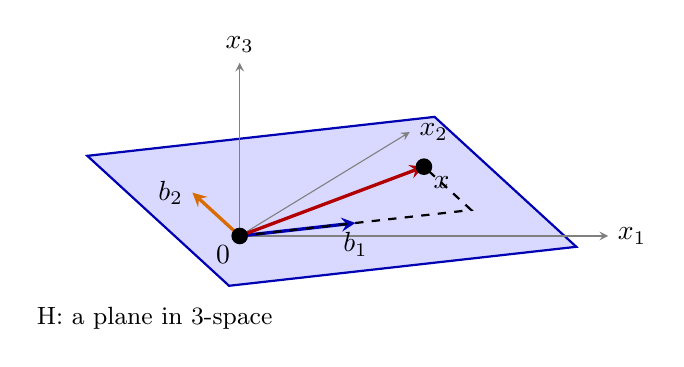
\begin{tikzpicture}[x=0.6cm,y=0.55cm,>=stealth]
  % oblique projection: the point (x1,x2,x3) is drawn at (x1+0.45*x2, x3+0.30*x2)
  % plane x1-2x2+x3=0 with b1=(2,1,0) and b2=(-1,0,1); corners are c1 b1 + c2 b2 for (c1,c2) = (-0.5,-1), (2.5,-1), (2.5,2), (-0.5,2)
  \fill[blue!15] (-0.225,-1.15)--(7.125,-0.25)--(4.125,2.75)--(-3.225,1.85)--cycle;
  \draw[thick,blue!70!black] (-0.225,-1.15)--(7.125,-0.25)--(4.125,2.75)--(-3.225,1.85)--cycle;
  \draw[->,gray] (0,0)--(7.8,0);
  \draw[->,gray] (0,0)--(3.6,2.4);
  \draw[->,gray] (0,0)--(0,4);
  \node[right] at (7.8,0) {$x_1$};
  \node[right] at (3.6,2.4) {$x_2$};
  \node[above] at (0,4) {$x_3$};
  \draw[->,very thick,blue!70!black] (0,0)--(2.45,0.3);
  \draw[->,very thick,orange!85!black] (0,0)--(-1,1);
  \draw[dashed,thick] (0,0)--(4.9,0.6)--(3.9,1.6);
  \draw[->,very thick,red!70!black] (0,0)--(3.9,1.6);
  \fill (3.9,1.6) circle (3pt);
  \node[below] at (2.45,0.3) {$b_1$};
  \node[left] at (-1,1) {$b_2$};
  \node[below right] at (3.9,1.6) {$x$};
  \fill (0,0) circle (3pt);
  \node[below left] at (0,0) {$0$};
  \node at (-1.8,-1.9) {\small H: a plane in 3-space};
\end{tikzpicture}
\end{center}

\textbf{Figure 2.} The plane $H$ of Example~\ref{ex:plane} (a patch of it) in the oblique picture of $\R^3$ used in Section 4.2, with the basis vectors $\bv{b}_1=(2,1,0)$ and $\bv{b}_2=(-1,0,1)$ in $H$ and the vector $\bv{x}=2\bv{b}_1+\bv{b}_2=(3,2,1)$, reached by two steps along $\bv{b}_1$ (dashed) and one along $\bv{b}_2$. The two basis vectors give $H$ the same kind of tilted grid as in Figure~1, now drawn on a plane inside $\R^3$.

\begin{think}{Coordinates are the free-variable values}{freevars}
In Example~\ref{ex:plane} the basis vectors came from the free variables $x_2$ and $x_3$, and $[\bv{x}]_{\mathcal{B}}=(2,1)$ for $\bv{x}=(3,2,1)$. Compare with the second and third entries of $\bv{x}$. Is this a coincidence? Explain using the form of the basis vectors in Procedure~\ref{4.3-proc:cond}, and then say how to read $[\bv{x}]_{\mathcal{B}}$ off any vector in $\Nul A$ without row reducing, if the basis is the one from Theorem~\ref{4.3-thm:nulbasis}.
\end{think}

\begin{exmp}{Coordinates in a null space}{nul}
Let $A=\begin{bmatrix}1&1&0&2\\0&0&1&-1\end{bmatrix}$. The free variables of $A\bv{x}=\bv{0}$ are $x_2,x_4$, with $x_1=-x_2-2x_4$, $x_3=x_4$, so $\Nul A$ has the basis $\mathcal{B}=\{\bv{b}_1,\bv{b}_2\}$ with $\bv{b}_1=(-1,1,0,0)$ and $\bv{b}_2=(-2,0,1,1)$ (Theorem~\ref{4.3-thm:nulbasis}). The vector $\bv{x}=(1,3,-2,-2)$ is in $\Nul A$: $A\bv{x}=(1+3+0-4,\ -2+2)=(0,0)$. Find $[\bv{x}]_{\mathcal{B}}$.

\textbf{Solution.}
\begin{align*}
\begin{amat}{cc|c}-1 & -2 & 1\\1 & 0 & 3\\0 & 1 & -2\\0 & 1 & -2\end{amat}
&\rops{R_1\leftrightarrow R_2}
\begin{amat}{cc|c}1 & 0 & 3\\-1 & -2 & 1\\0 & 1 & -2\\0 & 1 & -2\end{amat}
\rops{R_2+R_1}
\begin{amat}{cc|c}1 & 0 & 3\\0 & -2 & 4\\0 & 1 & -2\\0 & 1 & -2\end{amat}
\\[4pt]
&\rops{R_2\leftrightarrow R_3}
\begin{amat}{cc|c}1 & 0 & 3\\0 & 1 & -2\\0 & -2 & 4\\0 & 1 & -2\end{amat}
\rops{R_3+2R_2}
\begin{amat}{cc|c}1 & 0 & 3\\0 & 1 & -2\\0 & 0 & 0\\0 & 1 & -2\end{amat}
\\[4pt]
&\rops{R_4-R_2}
\begin{amat}{cc|c}1 & 0 & 3\\0 & 1 & -2\\0 & 0 & 0\\0 & 0 & 0\end{amat}
\end{align*}
So $[\bv{x}]_{\mathcal{B}}=(3,-2)$: $3\bv{b}_1-2\bv{b}_2=(-3+4,\ 3,\ -2,\ -2)=(1,3,-2,-2)$. \ $\checkmark$ These are the second and fourth entries of $\bv{x}$, the values of the free variables $x_2=3$, $x_4=-2$. The subspace $\Nul A$ lives in $\R^4$ and its coordinate vectors in $\R^2$.
\end{exmp}

\begin{exmp}{Coordinates in a column space}{col}
Let $A=\begin{bmatrix}1&2&0&1\\0&1&1&0\\1&3&1&1\end{bmatrix}$ with columns $\bv{a}_1,\dots,\bv{a}_4$ and let $\bv{b}=(5,2,7)$. The pivot columns of $A$ are columns $1$ and $2$ (the third row is the sum of the first two), so $\mathcal{B}=\{\bv{a}_1,\bv{a}_2\}$ is a basis for $\Col A$ (Theorem~\ref{4.3-thm:colbasis}). Find $[\bv{a}_3]_{\mathcal{B}}$, $[\bv{a}_4]_{\mathcal{B}}$ and $[\bv{b}]_{\mathcal{B}}$.

\textbf{Solution.} All three vectors are in $\Col A$ (the first two are columns of $A$, and $\bv{b}=\bv{a}_1+2\bv{a}_2$ is checked below), so row reduce once:
\begin{align*}
\begin{amat}{cc|ccc}1 & 2 & 0 & 1 & 5\\0 & 1 & 1 & 0 & 2\\1 & 3 & 1 & 1 & 7\end{amat}
&\rops{R_3-R_1}
\begin{amat}{cc|ccc}1 & 2 & 0 & 1 & 5\\0 & 1 & 1 & 0 & 2\\0 & 1 & 1 & 0 & 2\end{amat}
\\[4pt]
&\rops{R_3-R_2}
\begin{amat}{cc|ccc}1 & 2 & 0 & 1 & 5\\0 & 1 & 1 & 0 & 2\\0 & 0 & 0 & 0 & 0\end{amat}
\\[4pt]
&\rops{R_1-2R_2}
\begin{amat}{cc|ccc}1 & 0 & -2 & 1 & 1\\0 & 1 & 1 & 0 & 2\\0 & 0 & 0 & 0 & 0\end{amat}
\end{align*}
Reading the last three columns: $[\bv{a}_3]_{\mathcal{B}}=(-2,1)$, $[\bv{a}_4]_{\mathcal{B}}=(1,0)$ and $[\bv{b}]_{\mathcal{B}}=(1,2)$. Check: $-2(1,0,1)+(2,1,3)=(0,1,1)=\bv{a}_3$ and $(1,0,1)=\bv{a}_4=\bv{a}_1$ and $1(1,0,1)+2(2,1,3)=(5,2,7)=\bv{b}$. \ $\checkmark$ The coordinates of the non-pivot columns relative to the pivot columns are the entries of the reduced echelon form of $A$ (the weights that Example~\ref{4.3-ex:wrong} read off); the coordinate vector of $\bv{a}_4=\bv{a}_1$ is $\bv{e}_1$.
\end{exmp}

\begin{kc}{Coordinates in a plane}{plane}
Let $H$ and $\mathcal{B}=\{(2,1,0),(-1,0,1)\}$ be as in Example~\ref{ex:plane}. (a)~Find $[\bv{x}]_{\mathcal{B}}$ for $\bv{x}=(1,2,3)$ after checking that $\bv{x}$ is in $H$. (b)~Is $(1,1,1)$ in $H$? If so, find its coordinate vector. (c)~Is $(1,1,2)$ in $H$?
\end{kc}

\begin{think}{A plane and $\R^2$}{planer2}
The plane $H$ of Example~\ref{ex:plane} has the coordinate vector $[\bv{x}]_{\mathcal{B}}$ in $\R^2$ for each $\bv{x}$ in $H$. (a)~Is $H$ equal to $\R^2$? Is $H$ a subset of $\R^2$ (Pause and think~\ref{4.1-think:r2r3})? (b)~Which statements about adding and scaling vectors of $H$ can be moved to statements about vectors of $\R^2$? (c)~Can you think of a statement about vectors of $H$ that cannot be moved, one that depends on their having three entries?
\end{think}

\subsection*{Summary}
\begin{itemize}
  \item \textbf{Unique Representation.} If $\mathcal{B}=\{\bv{b}_1,\dots,\bv{b}_p\}$ is a basis for $V$, every $\bv{x}$ in $V$ is $c_1\bv{b}_1+\cdots+c_p\bv{b}_p$ for exactly one list of weights: spanning gives existence, independence gives uniqueness.
  \item \textbf{Coordinates.} $[\bv{x}]_{\mathcal{B}}=(c_1,\dots,c_p)$ in $\R^p$, with the basis in a fixed order; reordering the basis permutes the entries, and the same numbers name different vectors in different bases. $[\bv{b}_j]_{\mathcal{B}}=\bv{e}_j$, and $[\bv{x}]_{\mathcal{E}}=\bv{x}$ for the standard basis of $\R^n$.
  \item \textbf{Two directions.} Coordinates to vector: form the combination (no reduction). Vector to coordinates: row reduce $[\,\bv{b}_1\ \cdots\ \bv{b}_p\ \bv{x}\,]$. In $\R^n$ with $n$ basis vectors: $\bv{x}=P_{\mathcal{B}}[\bv{x}]_{\mathcal{B}}$ and $[\bv{x}]_{\mathcal{B}}=P_{\mathcal{B}}^{-1}\bv{x}$, with $P_{\mathcal{B}}$ invertible by the Invertible Matrix Theorem.
  \item \textbf{The coordinate mapping} is linear, one-to-one and onto $\R^p$ (an isomorphism). Linearity can be tested on numbers: one failed instance proves a map built from coordinates is not linear.
  \item \textbf{Using coordinates.} Independence, spanning, the basis property, membership in a span and vector equations in $\mathbb{P}_n$, $M_{2\times2}$ or a function space are decided by row reducing the matrix of coordinate vectors; dependence relations carry over with the same weights.
  \item \textbf{Subspaces of $\R^n$.} For a subspace $H$ with basis $\mathcal{B}$, $P_{\mathcal{B}}$ is not square, and $[\bv{x}]_{\mathcal{B}}$ is found by row reducing $[\,P_{\mathcal{B}}\ \bv{x}\,]$; an inconsistent system means $\bv{x}$ is not in $H$. For $\Nul A$ with the free-variable basis the coordinates are the values of the free variables; for $\Col A$ with the pivot columns they are the entries of the reduced echelon form.
\end{itemize}

\subsection*{Questions to think about before the next section}
\begin{enumerate}
  \item Two bases $\mathcal{B}$ and $\mathcal{C}$ of the same space give two coordinate vectors for the same $\bv{x}$ (Example~\ref{ex:samenums}(b)). Is $[\bv{x}]_{\mathcal{C}}$ determined by $[\bv{x}]_{\mathcal{B}}$ alone? Describe a way to compute it, and test it on the coordinate vectors of $(4,5)$ for $\mathcal{B}$ and $\mathcal{D}$.
  \item In Example~\ref{ex:plane} is there a $2\times3$ matrix $M$ with $M\bv{x}=[\bv{x}]_{\mathcal{B}}$ for every $\bv{x}$ in $H$? (Look at Pause and think~\ref{think:freevars}.)
  \item Suppose the columns of an $n\times n$ matrix $Q$ form a basis for $\R^n$. Prove that $Q$ is invertible. Conversely, if $Q$ is invertible, prove that its columns form a basis for $\R^n$ and find $[\bv{x}]_{\mathcal{B}}$ for this basis.
\end{enumerate}

\subsection*{Answers and discussion}
\begin{description}[leftmargin=0pt,itemsep=5pt]
  \item[Knowledge Check \ref{kc:fromto}.] (a)~$\bv{x}=2(3,1)-(1,2)=(6-1,\ 2-2)=(5,0)$. (b)~Solve $c_1(3,1)+c_2(1,2)=(7,4)$:
\begin{align*}
\begin{amat}{cc|c}3 & 1 & 7\\1 & 2 & 4\end{amat}
&\rops{R_1\leftrightarrow R_2}
\begin{amat}{cc|c}1 & 2 & 4\\3 & 1 & 7\end{amat}
\rops{R_2-3R_1}
\begin{amat}{cc|c}1 & 2 & 4\\0 & -5 & -5\end{amat}
\\[4pt]
&\rops{-\tfrac{1}{5}R_2}
\begin{amat}{cc|c}1 & 2 & 4\\0 & 1 & 1\end{amat}
\rops{R_1-2R_2}
\begin{amat}{cc|c}1 & 0 & 2\\0 & 1 & 1\end{amat}
\end{align*}
  so $[\bv{y}]_{\mathcal{B}}=(2,1)$. Check: $2(3,1)+(1,2)=(7,4)$. (c)~$p=2\cdot1+3(1+t)-1\cdot t^2=5+3t-t^2$.
  \item[Knowledge Check \ref{kc:inspect}.] (a)~$(4,6)=4(1,0)+2(0,3)$, so $[\bv{x}]_{\mathcal{B}}=(4,2)$. (b)~The third coordinate is the third entry, $c_3=1$. Then $x_2=c_2+c_3$ gives $c_2=2-1=1$, and $x_1=c_1+c_2+c_3$ gives $c_1=3-1-1=1$: $[\bv{x}]_{\mathcal{B}}=(1,1,1)$, which is $(1,0,0)+(1,1,0)+(1,1,1)=(3,2,1)$. (c)~$7-t^2=7\cdot1+0\cdot t-1\cdot t^2$, so $(7,0,-1)$. (d)~$\bv{x}=5\bv{b}_1+6\bv{b}_2+7\bv{b}_3=7\bv{b}_3+5\bv{b}_1+6\bv{b}_2$, so $[\bv{x}]_{\mathcal{C}}=(7,5,6)$.
  \item[Knowledge Check \ref{kc:PB}.] (a)~$P_{\mathcal{B}}=\begin{bmatrix}1&3\\2&5\end{bmatrix}$ with determinant $5-6=-1$, so $P_{\mathcal{B}}^{-1}=\begin{bmatrix}-5&3\\2&-1\end{bmatrix}$. Check: $\begin{bmatrix}1&3\\2&5\end{bmatrix}\begin{bmatrix}-5&3\\2&-1\end{bmatrix}=\begin{bmatrix}1&0\\0&1\end{bmatrix}$. (b)~$P_{\mathcal{B}}^{-1}\begin{bmatrix}1\\1\end{bmatrix}=\begin{bmatrix}-2\\1\end{bmatrix}$, and $-2(1,2)+1(3,5)=(1,1)$. \ $\checkmark$ (c)~$P_{\mathcal{B}}$ takes a coordinate vector to the vector; $P_{\mathcal{B}}^{-1}$ takes a vector to its coordinate vector.
  \item[Knowledge Check \ref{kc:outside}.] (a)~$p=2\cdot1+0(1+t)-1(1+t)^2=2-(1+2t+t^2)=1-2t-t^2$. (b)~$A=2E_{11}-E_{12}+0E_{21}+5E_{22}$, so $[A]=(2,-1,0,5)$. (c)~The standard coordinates of $\sin t$ are $(0,1)$; solving $c_1(1,1)+c_2(1,-1)=(0,1)$ gives $c_1=\tfrac12$, $c_2=-\tfrac12$: $[h]_{\mathcal{C}}=(\tfrac12,-\tfrac12)$. Check: $\tfrac12(\cos t+\sin t)-\tfrac12(\cos t-\sin t)=\sin t$.
  \item[Knowledge Check \ref{kc:testkc}.] (a)~The coordinate vectors $(1,0,1,0)$, $(0,1,0,1)$, $(1,1,1,1)$: the third is the sum of the first two, so the set is dependent, with $(1+t^2)+(t+t^3)-(1+t+t^2+t^3)=0$. (b)~The coordinate vectors $(1,0,0,1)$, $(0,1,-1,0)$, $(1,1,-1,1)$: the third is the sum of the first two, so dependent: $I+K-N=\mathbf{0}$. (c)~The standard coordinates are $(1,1,0)$, $(0,1,1)$, $(1,0,1)$, $(1,1,1)$:
\begin{align*}
\begin{amat}{cccc}1 & 0 & 1 & 1\\1 & 1 & 0 & 1\\0 & 1 & 1 & 1\end{amat}
&\rops{R_2-R_1}
\begin{amat}{cccc}1 & 0 & 1 & 1\\0 & 1 & -1 & 0\\0 & 1 & 1 & 1\end{amat}
\rops{R_3-R_2}
\begin{amat}{cccc}1 & 0 & 1 & 1\\0 & 1 & -1 & 0\\0 & 0 & 2 & 1\end{amat}
\end{align*}
  There is a pivot in every row, so the coordinate vectors span $\R^3$ and the four polynomials span $\mathbb{P}_2$ (Theorem~\ref{thm:transfer}(c)). They are not independent, because four vectors in $\R^3$ cannot be (Theorem~\ref{1.7-thm:count}).
  \item[Knowledge Check \ref{kc:plane}.] (a)~$1-4+3=0$, so $\bv{x}$ is in $H$. The coordinates are the second and third entries (Pause and think~\ref{think:freevars}): $[\bv{x}]_{\mathcal{B}}=(2,3)$. Check: $2(2,1,0)+3(-1,0,1)=(4-3,\ 2,\ 3)=(1,2,3)$. \ $\checkmark$ (b)~$1-2+1=0$, so yes: $(1,1,1)=(2,1,0)+(-1,0,1)$, $[\,(1,1,1)\,]_{\mathcal{B}}=(1,1)$. (c)~$1-2+2=1\neq0$: no.
  \item[Pause and think \ref{think:hyp}.] (a)~Spanning gives existence (some combination equals $\bv{x}$); independence gives uniqueness (the difference of two representations is a dependence relation, which must be trivial). (b)~If the set spans but is dependent, some vectors have several representations, as in Example~\ref{ex:contrast}(a), where $(3,2)=3\bv{e}_1+2\bv{e}_2=\bv{e}_1+2\bv{s}$. (c)~If the set is independent but does not span, some vectors have no representation, as $(0,0,1)$ in Example~\ref{ex:contrast}(b).
  \item[Pause and think \ref{think:ordered}.] $[\bv{x}]_{\mathcal{B}}=(5,7)$ and $[\bv{x}]_{\mathcal{C}}=(7,5)$: the same weights listed in the order of the basis vectors. If we were free to list the weights in any order, the symbol $[\bv{x}]_{\mathcal{B}}$ would not name a single vector of $\R^p$ (it could be $(5,7)$ or $(7,5)$), the coordinate mapping would not be a function, and two coordinate vectors could not be compared or added meaningfully. A basis used for coordinates therefore comes with its order.
  \item[Pause and think \ref{think:square}.] (a)~The columns of $P_{\mathcal{B}}$ are linearly independent (independence of $\mathcal{B}$) and span $\R^n$ (spanning). (b)~Statements (e) (``the columns of $A$ form a linearly independent set'') and (h) (``the columns of $A$ span $\R^n$''); each alone implies invertibility once the matrix is square, so a basis gives both. (c)~A matrix that is not square has no inverse (the definition of invertible requires a square matrix, Definition~\ref{2.2-def:inverse}), so the formula $[\bv{x}]_{\mathcal{B}}=P_{\mathcal{B}}^{-1}\bv{x}$ would not make sense. The formula $\bv{x}=P_{\mathcal{B}}[\bv{x}]_{\mathcal{B}}$ would still hold, since it is only a restatement of $\bv{x}=c_1\bv{b}_1+\cdots+c_p\bv{b}_p$; and the coordinates could still be found by row reducing $[\,P_{\mathcal{B}}\ \bv{x}\,]$, as in the plane example below.
  \item[Pause and think \ref{think:notpreserved}.] (a)~No: $\bv{x}=(4,5)$ and $[\bv{x}]_{\mathcal{B}}=(3,2)$ are different vectors (they are not even in the same space, in general). (b)~No: $(1,0)$ has positive-or-zero entries, but $[\,(1,0)\,]_{\mathcal{B}}=(\tfrac13,-\tfrac13)$ has a negative entry. Positivity of entries is not preserved. (c)~The first can be tested in coordinates, because it uses only addition: $\bv{u}=\bv{v}+\bv{w}$ if and only if $[\bv{u}]_{\mathcal{B}}=[\bv{v}]_{\mathcal{B}}+[\bv{w}]_{\mathcal{B}}$ (the map is linear and one-to-one). The second refers to the entries themselves, which change with the basis, and cannot.
  \item[Pause and think \ref{think:transfer}.] (a)~Linearity, in the form $[c_1\bv{u}_1+\cdots+c_k\bv{u}_k]_{\mathcal{B}}=c_1[\bv{u}_1]_{\mathcal{B}}+\cdots+c_k[\bv{u}_k]_{\mathcal{B}}$. (b)~One-to-one: $[\bv{p}]_{\mathcal{B}}=\bv{0}=[\bv{0}]_{\mathcal{B}}$ forces $\bv{p}=\bv{0}$. (c)~If $T$ were linear but not one-to-one, some nonzero polynomial would have $T(\bv{p})=\bv{0}$, and a set of independent polynomials containing it, or a combination of independent polynomials that $T$ sends to zero, could have dependent images. So the direction ``the polynomials are independent, hence their images are independent'' fails; the direction ``the images are independent, hence the polynomials are independent'' holds for every linear map. One-to-one is what makes both directions hold.
  \item[Pause and think \ref{think:freevars}.] It is not a coincidence. In Procedure~\ref{4.3-proc:cond} and Theorem~\ref{4.3-thm:nulbasis}, the basis vector $\bv{b}_j$ for the free variable $x_{i_j}$ has a $1$ in position $i_j$ and a $0$ in the positions of the other free variables. So a vector $\bv{x}=c_1\bv{b}_1+\cdots+c_p\bv{b}_p$ has $x_{i_j}=c_j$: the entry of $\bv{x}$ in the position of the $j$th free variable is the $j$th coordinate. Hence $[\bv{x}]_{\mathcal{B}}$ is read off $\bv{x}$ by picking the entries in the free-variable positions, with no row reduction. In Example~\ref{ex:plane} these are the second and third entries of $(3,2,1)$, namely $(2,1)$; in Example~\ref{ex:nul}, the second and fourth entries of $(1,3,-2,-2)$, namely $(3,-2)$. This works only for the free-variable basis and only for vectors already known to be in the subspace.
  \item[Pause and think \ref{think:planer2}.] (a)~No: the vectors of $H$ have three entries, those of $\R^2$ two, so $H\neq\R^2$; and $H$ is not a subset of $\R^2$ either (compare Pause and think~\ref{4.1-think:r2r3}). The coordinate mapping is a correspondence between two different spaces. (b)~Every statement that is built from addition and scalar multiplication: that $\bv{u}$ is a combination of $\bv{v}$ and $\bv{w}$, that a set of vectors of $H$ is independent or spans $H$ (Theorem~\ref{thm:transfer}). (c)~Statements that depend on the entries: ``the third entry of $\bv{x}$ is $1$'', or ``$\bv{x}$ is also a solution of $x_1+x_3=2x_2$'' (which is true for all of $H$ but is a statement about three entries). Such statements have no meaning for a vector of $\R^2$.
  \item[Before the next section.] (1)~Yes. The vector $\bv{x}$ is determined by $[\bv{x}]_{\mathcal{B}}$, namely $\bv{x}=P_{\mathcal{B}}[\bv{x}]_{\mathcal{B}}$ (when both bases are bases for $\R^n$), and $[\bv{x}]_{\mathcal{C}}=P_{\mathcal{C}}^{-1}\bv{x}$ is determined by $\bv{x}$. For $\mathcal{B}=\{(2,1),(-1,1)\}$ and $\mathcal{D}=\{(1,1),(1,-1)\}$ and $[\bv{x}]_{\mathcal{B}}=(3,2)$: $\bv{x}=(4,5)$, and solving $c_1+c_2=4$, $c_1-c_2=5$ gives $[\bv{x}]_{\mathcal{D}}=(\tfrac92,-\tfrac12)$, as in Example~\ref{ex:samenums}. (2)~Yes: $M=\begin{bmatrix}0&1&0\\0&0&1\end{bmatrix}$ picks out the second and third entries, which are the coordinates by Pause and think~\ref{think:freevars}; $M(3,2,1)=(2,1)$. It does not matter that $M$ is not invertible: it is defined on $\R^3$, and only its action on $H$ gives coordinates. (3)~If the $n$ columns of $Q$ form a basis for $\R^n$, then $Q=P_{\mathcal{B}}$ is invertible by Theorem~\ref{thm:PB}. Conversely, if $Q$ is invertible, its columns are independent and span $\R^n$ by Theorem~\ref{2.3-thm:imt}, so they form a basis $\mathcal{B}$; then $Q=P_{\mathcal{B}}$ and $[\bv{x}]_{\mathcal{B}}=Q^{-1}\bv{x}$.
\end{description}

\end{document}
